\chapter{ISR Simulation}
\label{chapter:stisrs}
\thispagestyle{myheadings}

% set this to the location of the figures for this chapter. it may
% also want to be ../Figures/2_Body/ or something. make sure that
% it has a trailing directory separator (i.e., '/')!
\graphicspath{{4_STISRS/Figures/}}

%%%%%%%%%%%%%%%%%%%%%%%%%%%%%%%%%%%%%%%%%%%%%%%%%%%%%%%%%%%%%%%%%%%%%%%%%

The previous chapter developed a forward model for the ISR sensing modality, valid for an arbitrary beam pattern and a target that may vary in space and time.   As described, the collected signal in ISR is noise-like with the variance of the fitted parameters directly dependent on the length of temporal integration.   Therefore, evaluation of any inverse theoretic scheme requires a full simulation of the ISR acquisition. The following chapter details the methodology behind SimISR along with some processed examples. The first section shows how the synthetic data is created at complex voltage level. After which results of these simulations are shown after the data has been processed as described in Section \ref{section:isrproc}. The results are interpolated back to the original Cartesian space of the plasma parameters. 

\section{Simulation Methodology}
\label{sec:simmeth}
The SimISR software package allows one to analyze different  experiment scenarios by simulating the ISR measurement process. %The space-time ambiguity is modeled using a coordinate transform and the pulse as a window along range while the statistical error is taken into account by creating complex shaped Gaussian noise.  
% JOHN:   The above  sentence seems unclear.  Is the adjusted version below accurate?  
% Josh: That is correct, although I have to make sure I mention the use of the pulse as a window function that creates the range ambiguity. I believe I do this later on but I have to check.
The space-time ambiguity is modeled through a three-dimensional blurring kernel along with appropriate coordinate transformations to account for target variation during radar acquisition.   The statistical error is taken into account by creating complex shaped Gaussian noise.    
In what follows, we begin with a description of construction of spectral filters designed to create the noise-like signal received in ISR experiments. This is followed by description of the process of creating complex receiver voltage data. The last portion details the processing used to create statistical estimates of ACFs.

\subsection{Creating Filters}

The simulator takes as input a discretized set of ionosphere state parameters in Cartesian coordinates which can vary in time. These state parameters electron density ($N_e$), electron temperature ($T_e$), ion temperatures for each ion species ($T_i$) the densities for each ion species. This corresponds to the true field we seek to reconstruct. The first step in the simulator is to create theoretical ISR spectra at each point from the prescribed parameters. For details on calculating these spectra from the intrinsic plasma parameters see, Section~\ref{sec:incohscat}, and Appendix~\ref{appendix1} for greater detail. 

Once the spectra have been created, the simulator transforms the resulting values to a radar-centered spherical coordinate system. This coordinate change acts as a linear operator in spatial dimensions, and the spectra are accordingly weighted and averaged. The weighting in azimuth and elevation is determined by the antenna beam pattern, while the weighting in range (i.e. along beam) is simply a binary test of whether the spectra are within the range gate. If there are no spectra within the range gate, a nearest neighbor rule is used which selects the closest point in Cartesian space. This method to create the spectra for each point is an acceptable approximation because spatial correlations between the electron density fluctuations will be on the order of the Debye length \citep{farley1969} which is, in nearly all practical cases, significantly smaller than the beam width or range gate size. This is same as making the assumption of wide-sense stationarity with uncorrelated scattering (WSSUS) \citep{Kailath:1962jx}. The algorithm implementing spatial sampling is shown in the simplified diagram in Figure~\ref{fig:beamdia}.

\begin{figure}[!t]
\centering
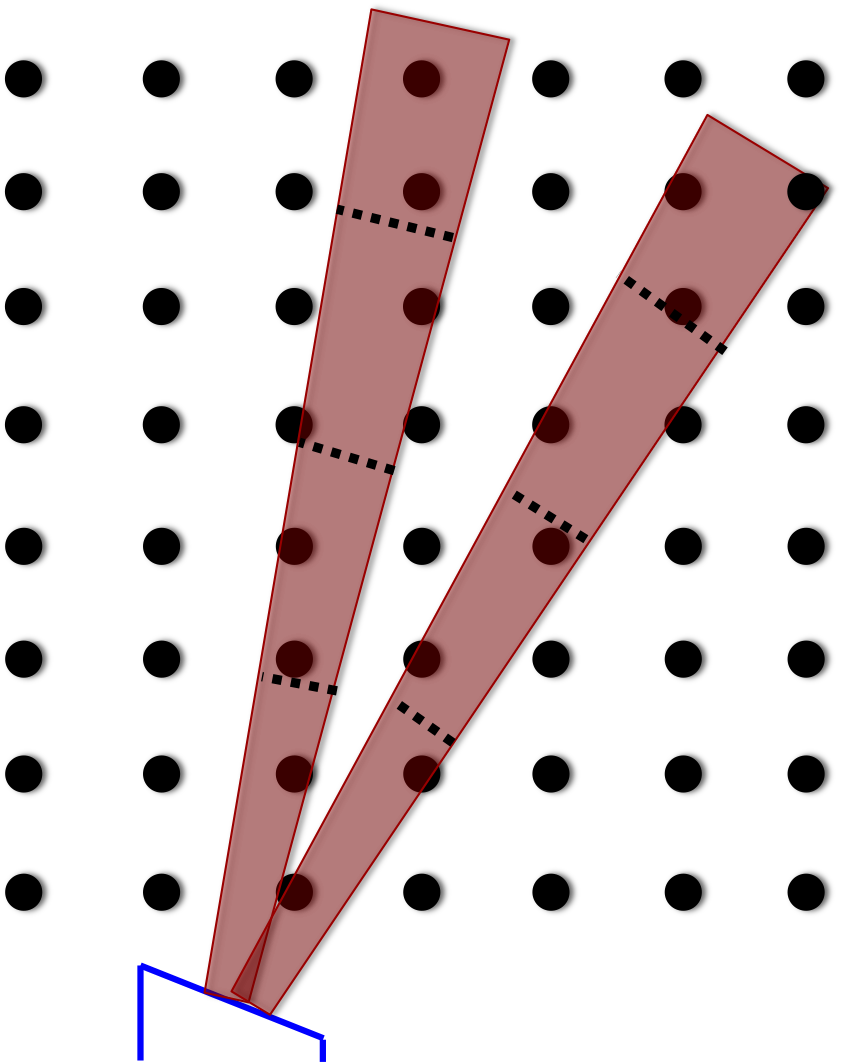
\includegraphics[width=2in]{beamsampling}
\caption{Each point is a from a discrete sampling of a Cartesian space. The beams are broken up into range gates, separated by the dotted lines, and the parameters at each point overlapping within these gates are averaged.}
\label{fig:beamdia}
\end{figure}
 
% Once the spectrum at the specific point in range and angle space has been determined, the filter $H_m(\omega)$, is created by simply taking the square root of the spectrum, $S_m(\omega | \: \bm{\theta})$,

% \begin{equation}
% \label{eq1}
% H_m(\omega) = \sqrt{S_m(\omega | \: \bm{\theta})}.
% \end{equation}

Once the theoretical spectrum for a given scattering volume has been calculated, an appropriate spectral shaping filter is created. The method to create the filter given a desired spectrum or ACF can be done in a number of ways \citep{Kasdin:1995wi}. The implementation in SimISR creates an infinite impulse response filter in order to ensure a causal, minimum phase filter. 
%% PJE: Why does SimISR pick an IIR filter, which is not guaranteed to have a linear phase response across the passband (i.e. constant delay)?  Might be worth a comment here.
%% JPS: This creates a causal, minimum phase filter. It may not be linear phase but its not necessarily need in this application as we are not worried about dispersion of the input signal. The filters just need to be stable and the causality allows one to use the minimum phase assumption to justify stability.
The coefficients are determined using the ACF by solving the following set of equations,

\begin{equation}
\label{eq:filtereq}
\begin{bmatrix} R_m(0) & R_m(L-1)& \cdots & R_m(1) \\ 
R_m(1) & R_m(0)& \cdots & R_m(2)\\ 
\vdots & &\ddots  & \vdots \\  
R_m(L-1) & R_m(L-2) & \cdots & R_m(0) 
\end{bmatrix}
 \left[ \begin{array}{c} a_1\\ a_2\\\vdots \\ a_L \end{array} \right]=\left[ \begin{array}{c} R_m(1) \\ R_m(2)\\ \vdots \\R_m(L) \end{array} \right]
\end{equation}

\noindent where $R_m(l)$ are the ACF values, $L$ is the desired length of the filter, and $ a_i$ are the set of filter coefficients. The filter then takes the form in the frequency domain as the following,

\begin{equation}
\label{eq:filtz}
H_m(z) = \frac{G}{1-\displaystyle \sum_{l=1}^{L} a_l z^{-l}}.
\end{equation}
\noindent The gain term $G$ is used to make sure the noise has the correct variance. This can be calculated as 

\begin{equation}
\label{eq:gainterm}
G=\sqrt{\displaystyle \sum_{l=0}^L -a_l R_m(l)},
\end{equation}

\noindent where $a_0=-1$. This method has been used in similar ways in other contexts--e.g., the creation of vocoders for speech processing applications, as it creates causal and stable infinite impulse response filters \citep{rabinerdigitalspeech}. Equivalently, this technique is creating an autoregressive (AR) process. Alternatively a moving average (MA) process could be use, which would result in a finite impulse response filter but calculating the coefficients for this filter can be much more computationally difficult \citep{kayvol1} .
%\noindent The term $ \bm{\theta}$ refers to the plasma parameters needed to make the spectrum. This filter then is used to create the synthetic IQ data.

\subsection{Simulated Complex Voltage Creation}

The algorithm used to create sampled complex receiver voltages employs a complex white Gaussian noise (CWGN) process (``plant") that is spectrally shaped at its output using a time domain filter. As stated in the previous subsection, each point in space and time will have a separate noise plant and filter which is derived from the plasma and radar parameters parameters. Figure \ref{fig:IQdiagram} presents a representative example. 

\begin{figure}[h!]
\centering
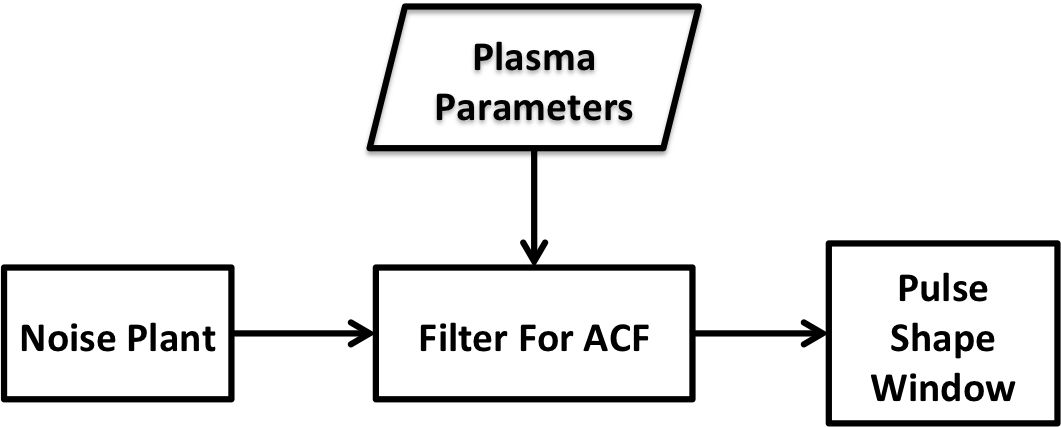
\includegraphics[width=4in]{diagrampart}
\caption{Diagram for main kernel of complex receiver voltage simulator signal flow.}
\label{fig:IQdiagram}
\end{figure}

The creation of one set of complex receiver voltage data can be represented by

\begin{equation}
\label{eq2}
y_m (k)= s(k)\left[h_m(k)*w(k)\right],
\end{equation}
 
\noindent where $s(k)$ is the overall transmitted pulse envelope, $h_m(k)$ is the time domain representation of the filter in Equation \ref{eq:filtz} and $w(k)\sim CN(0,\mathbf{I})$ or CWGN noise process. The pulse shape acts as a window function, since the plasma will only reflect energy during the time it is illuminated by the radar signal. 
%The application of this filter is actually done in the frequency domain. This is possible because the Discrete Fourier Transform (DFT) of a vector of CWGN is also CWGN. The only difference is that there is a change in the variance, which is tied to the number of points used in the DFT \citep{kayvol1}. With this in mind Equation \ref{eq2} can be implemented as the following,

%\begin{equation}
%\label{eq:fftfilt}
%y_m (k)= s(k)\displaystyle \sum_{i=0}^{K-1}e^{j\omega_ik}\left[ \sqrt{S_m(\omega_i | \: \bm{\theta})}w(\omega_i)\right],
%\end{equation}
%
%\noindent where $\omega_i$ is the frequency variable, $w(\omega_i) \sim CN(0,\mathbf{I})$ and $K$ is the number of points used for the DFT \citep{michellnoisesim1981}.

After the data for each range gate $y_m(k)$ is created, the received signal's power can be calculated from ISR plasma scattering theory as 

\begin{equation}
\label{eq3}
P_r = \frac{\left(c\Delta T\right) G \lambda^2}{2(4\pi)^2}\frac{P_t }{R^2}\frac{\sigma_e N_e}{(1+k^2\lambda_D^2),(1+k^2\lambda_D^2 + T_r)},
\end{equation}
 
 \noindent where $P_r$ is the power received in Watts (W), $k$ is the wavenumber of the radar in meters (m), $c$ is the speed of light in m/s, $\Delta T$ is the along-range gate extent in seconds, $G$ is the gain of the antenna, $P_t$ is the power of the transmitter in W, $\sigma_e$ is the electron radar cross section in $m^2$,  $\lambda_D$ is the Debye length in m, $N_e$ is the electron density in m$^{-3}$, and $T_r$ is the electron to ion temperature ratio.
  
The received signal power calculated at each range gate using Equation~\ref{eq3} is used as a scaling constant for each $y_m(k)$ series.  A delayed and summed operator yields a model of the received radar scatter signal:
 
\begin{equation}
\label{eq4}
x(n) = \displaystyle\sum\limits_{m =0}^{M-1} \alpha(m)y_m(n-m),
\end{equation}

\noindent where $\alpha(m) = \sqrt{P_r(m)}/\widehat{\sigma}_y$ and $\widehat{\sigma}_y$ is the estimate of the standard deviation of $y_m(k)$. Each signal from each $M$ number of range gates is assumed independent of one and other as this would violate the assumption that any spatial correlations drop off much faster than the distance covered by one range gate, see Section ~\ref{sec:sptimeamb}. Lastly, to model total noise from the radar system and environment, an additive CWGN process is included, creating the final simulated complex receiver voltage sequence

\begin{equation}
\label{eq:addnoise}
x_f(n) = x(n) +\sqrt{\frac{k_bT_{sys}B}{2}} w(n), \quad w(k)\sim CN(0,\mathbf{I})
\end{equation}

\noindent where $k_b$ is Boltzmann's constant, $T_{sys}$ is the system temperature and $B$ is the system bandwidth.
A full diagram of the model can be seen in Figure \ref{fig:isrdiag}.

\begin{figure}[!h]
\centering
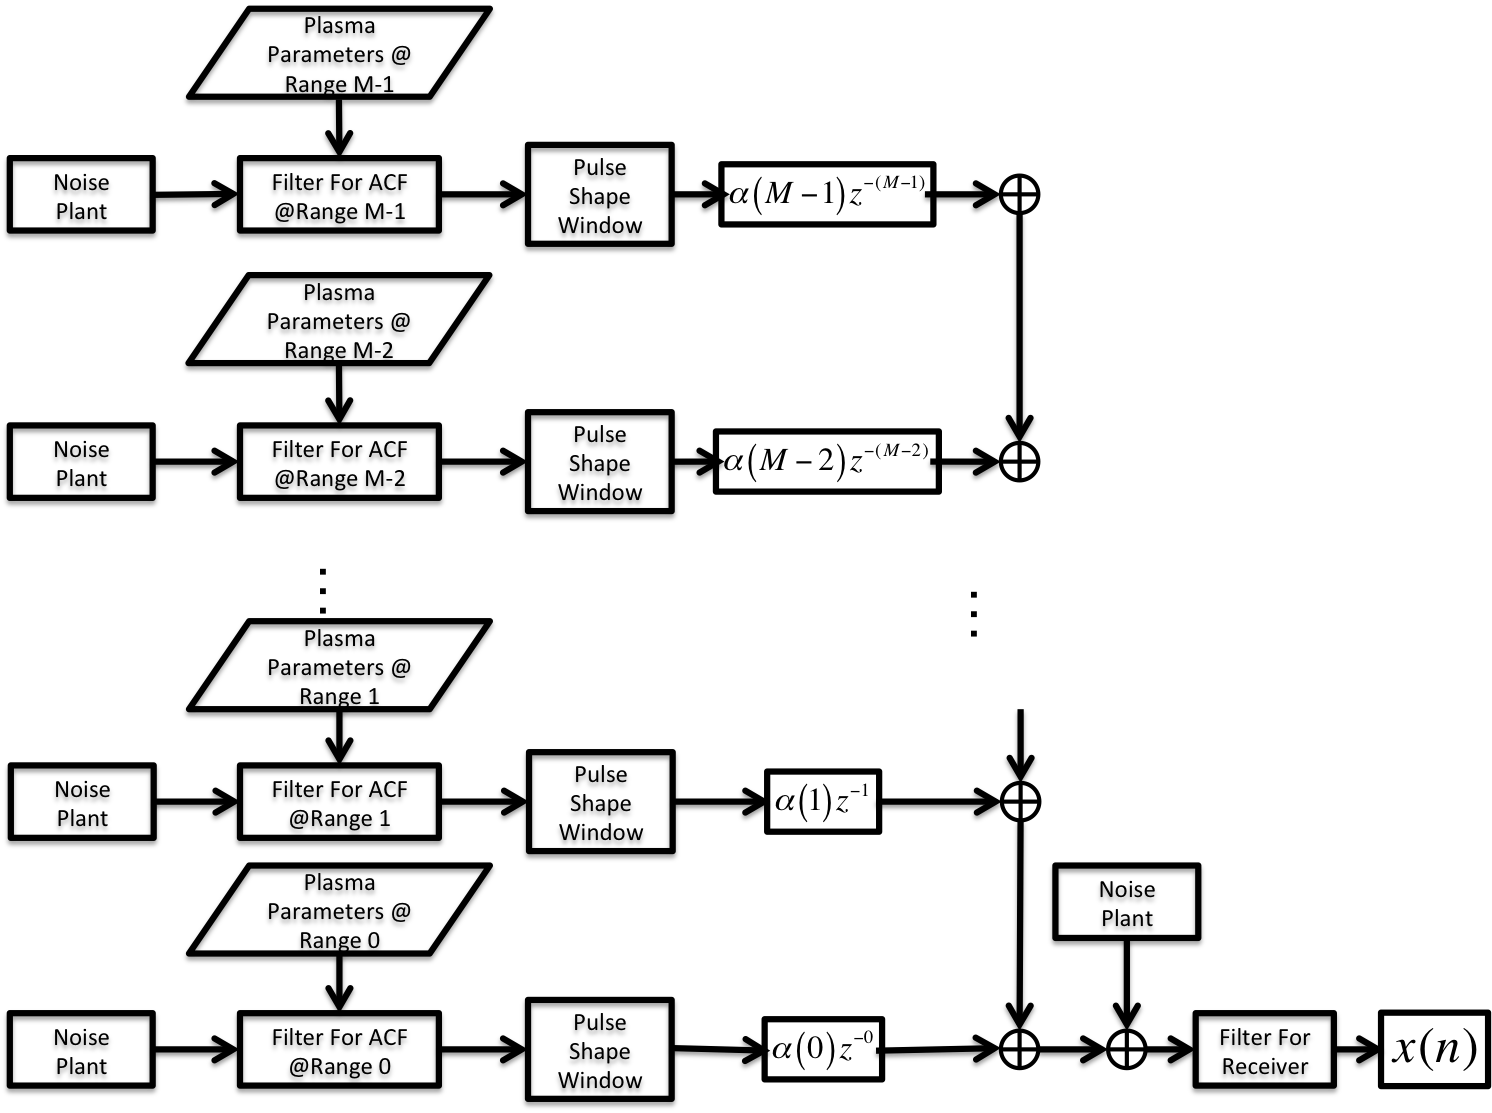
\includegraphics[width=5.5in]{diagram}
\caption{Full SimISR signal flow diagram where the diagram from Figure~\ref{fig:IQdiagram} is replicated for each range gate. The signals for each range gate are then weighted and then summed together to form the data from a single beam. Also note that each noise plant is assumed independent of one and other.}
\label{fig:isrdiag}
\end{figure}

\section{Simulation Examples}
\label{sec:simex}

The framework for SimISR allows exploration of a number of aspects of ISR processing. Within the scope of this article, we will focus on four application examples.

The first example compares the output of SimISR with a set of relatively geophysically quiet data from the PFISR system. The next case demonstrates how the simulator can be used for Monte Carlo estimates of ISR spectra. In this case, we hold all of the plasma parameters constant and determine how the distribution of the measured parameters evolve. The next example uses a simple altitude distribution of ionospheric plasma parameters to show the impact of the forward model of the ISR on a basic measurement of electron density. This is intended to illustrate that basic ambiguities inherent in ISR measurements can give the appearance of a change in morphology of the plasma phenomena when none truly exists. Finally, the output of a fully consistent multi-fluid ionosphere model is used as input to the ISR simulator and is applied in two use cases relevant to experiment planning, one varying over two spatial dimensions and another varying in all three spatial dimensions. The results of these use cases illustrate an inherent tradeoff in experiment construction between reducing statistical fluctuations in the measurement and increasing distortion in the final reconstruction. 

\subsection{Real Data Comparison}

The first example shows PFISR data compared to SimISR. This comparison is made up of an altitude profile taken from PFISR during a geophysically quiescent period during the day. An input set of parameters was created using analytic functions that resemble the data from the radar. The functional forms used are a Chapman function for the electron density; arctan functions for the ion and electron temperatures; and a constant of zero for the ion velocities.

The chosen parameters for the inputs can be seen in Figure \ref{fig:simisrparamcomp} as the green lines. The collected PFISR data can be seen in blue and the SimISR output in red. The plots show that the PFISR and SimISR data show similar variability within the parameters although SimISR starts to have bias in the electron and ion temperatures above 500 km. The $T_i$ and $T_e$ are negatively correlated so any change in one would create the opposite effect in the other parameter.


\begin{figure}[h!]
\centering
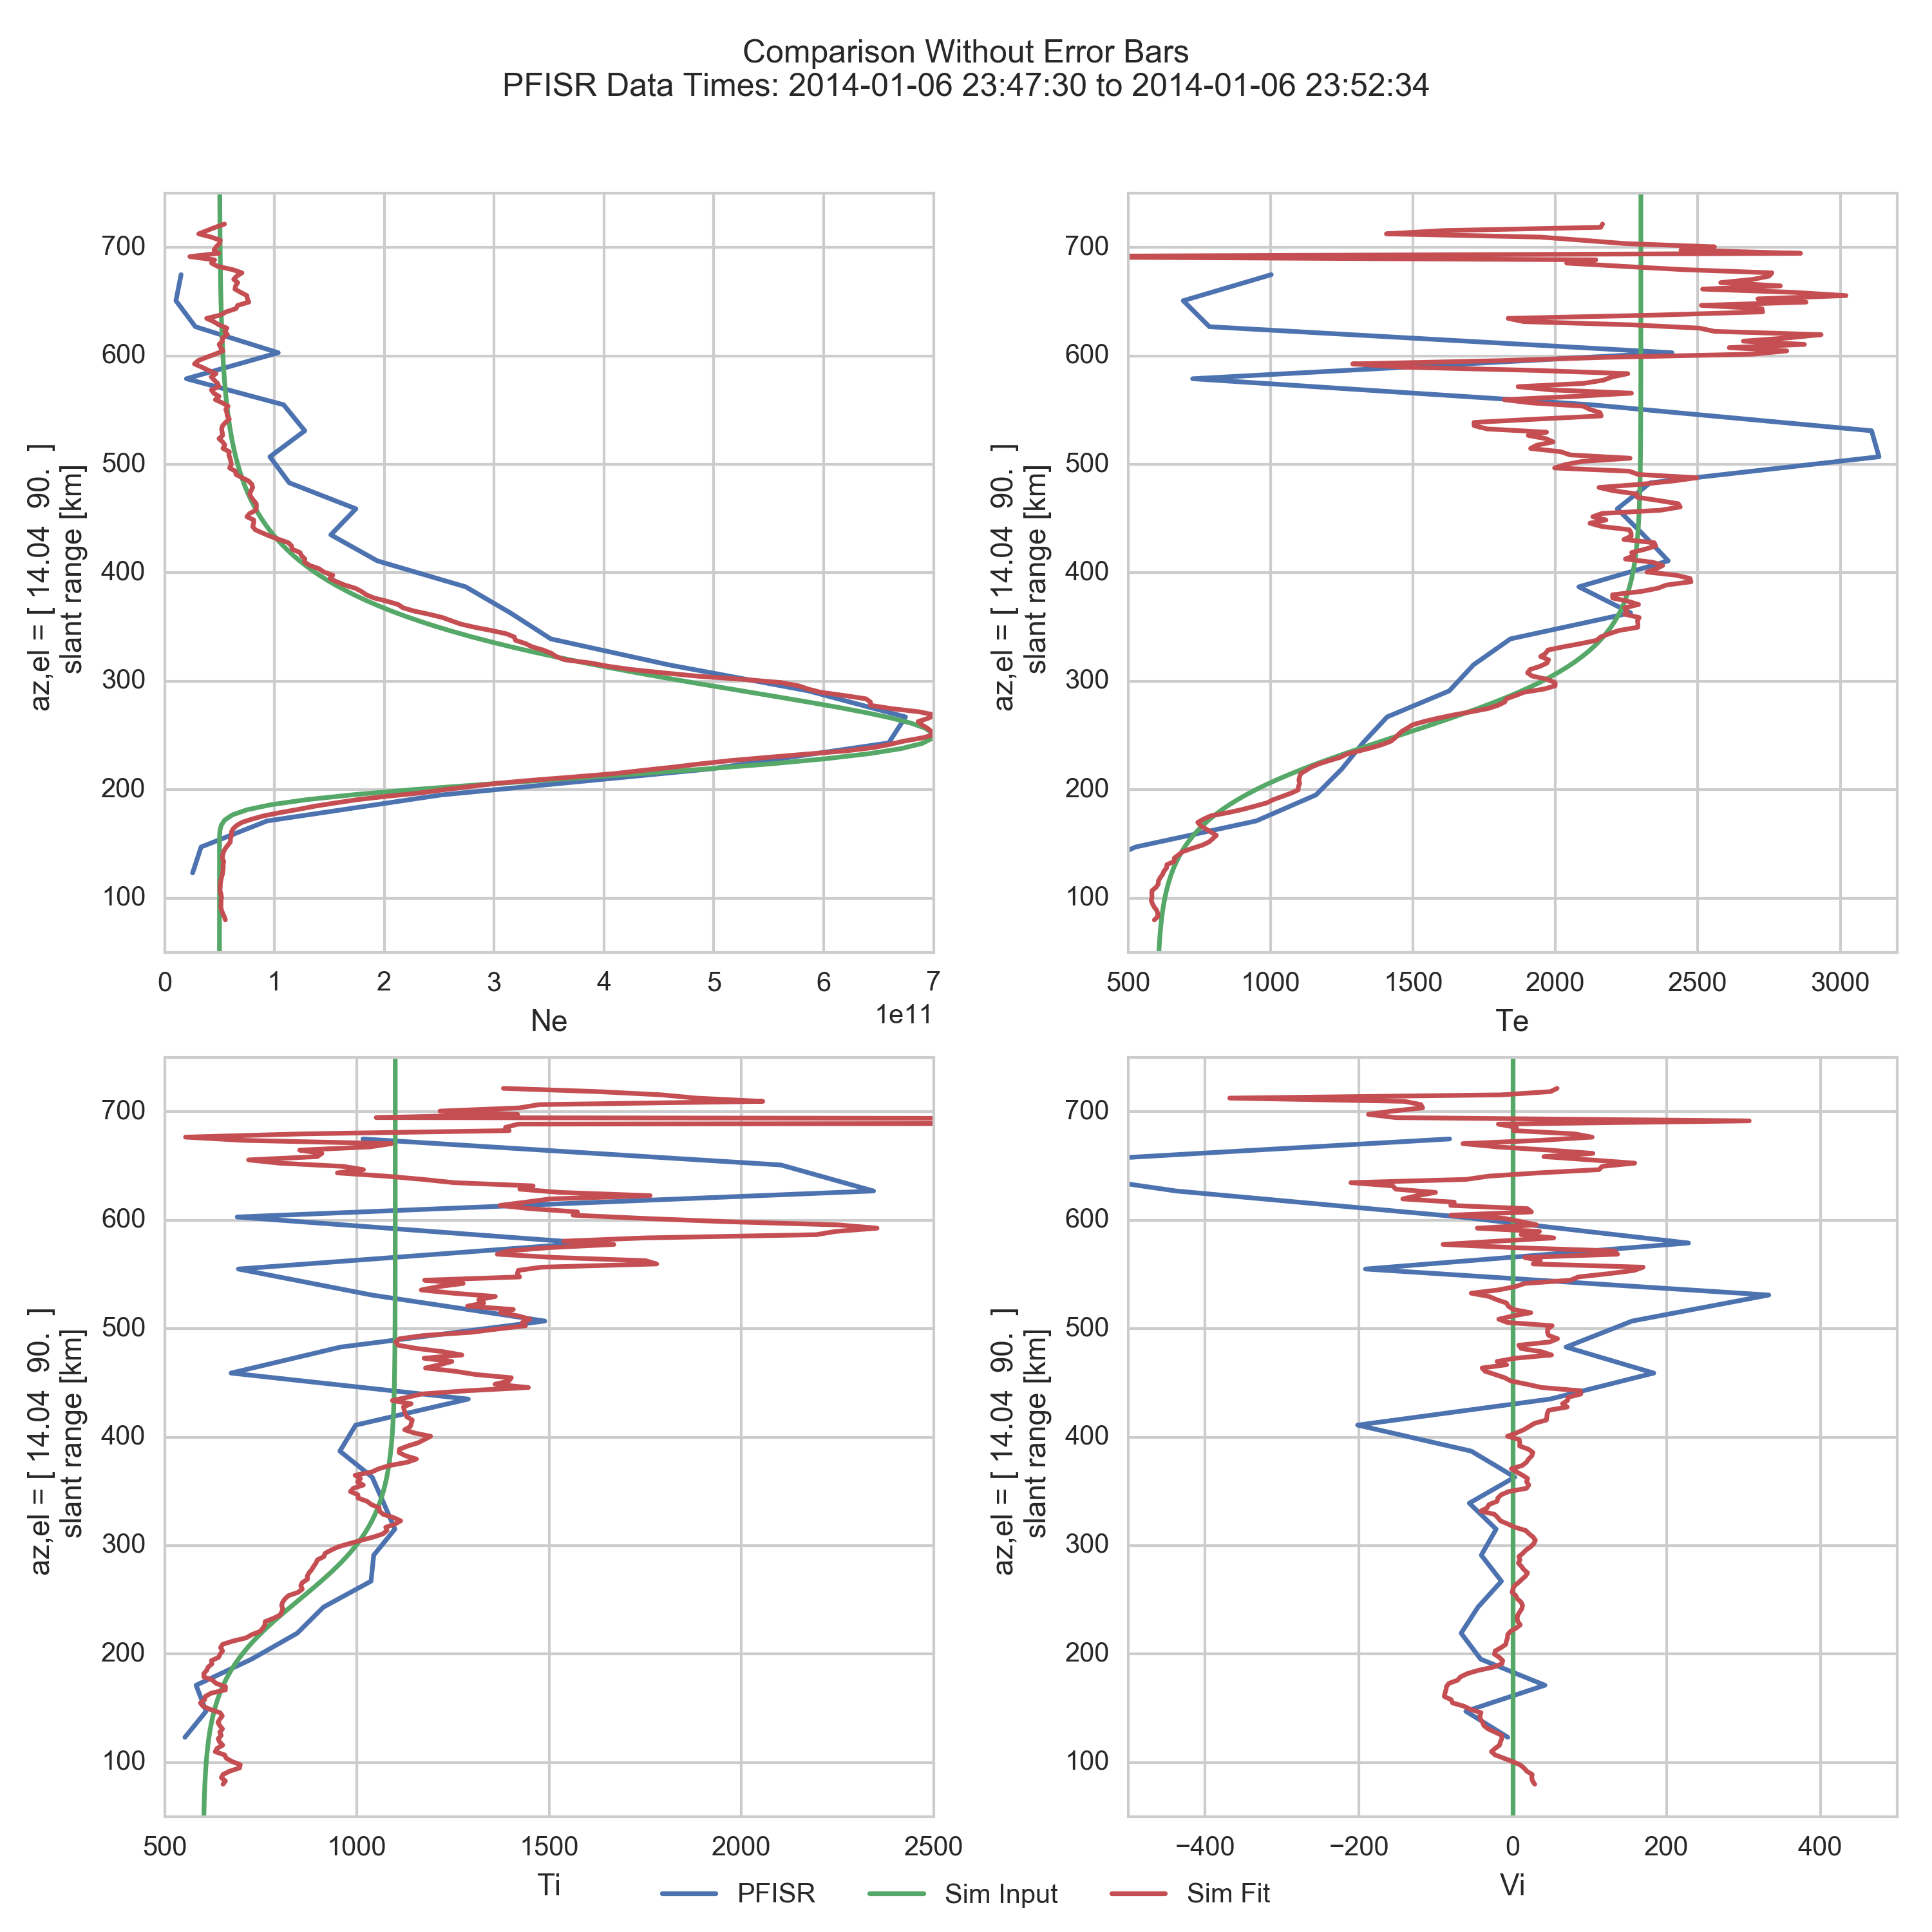
\includegraphics[width=4.5in]{Paramcomp}
\caption{Comparison of real data from PFISR, in blue, with SimISR data, in red, and an input parameter distribution in green.}
\label{fig:simisrparamcomp}
\end{figure}

A version of Figure \ref{fig:simisrparamcomp} can be seen with error bars in Figure \ref{fig:simisrparamcompeb}. The error bars in the SimISR parameters seem to be much small than those from PFISR. This seems to be due to a number of reason: the first is that there are slightly different fitting algorithms used between PFISR and SimISR; second PFISR has to fit data which is created through multiple ion species, thus creating a larger source of uncertainty if the ion species relative contributions are incorrect; lastly there are other sources of error that PFISR operators may add into the their uncertainty calculations that are not present in a simulation. 

\begin{figure}[h!]
\centering
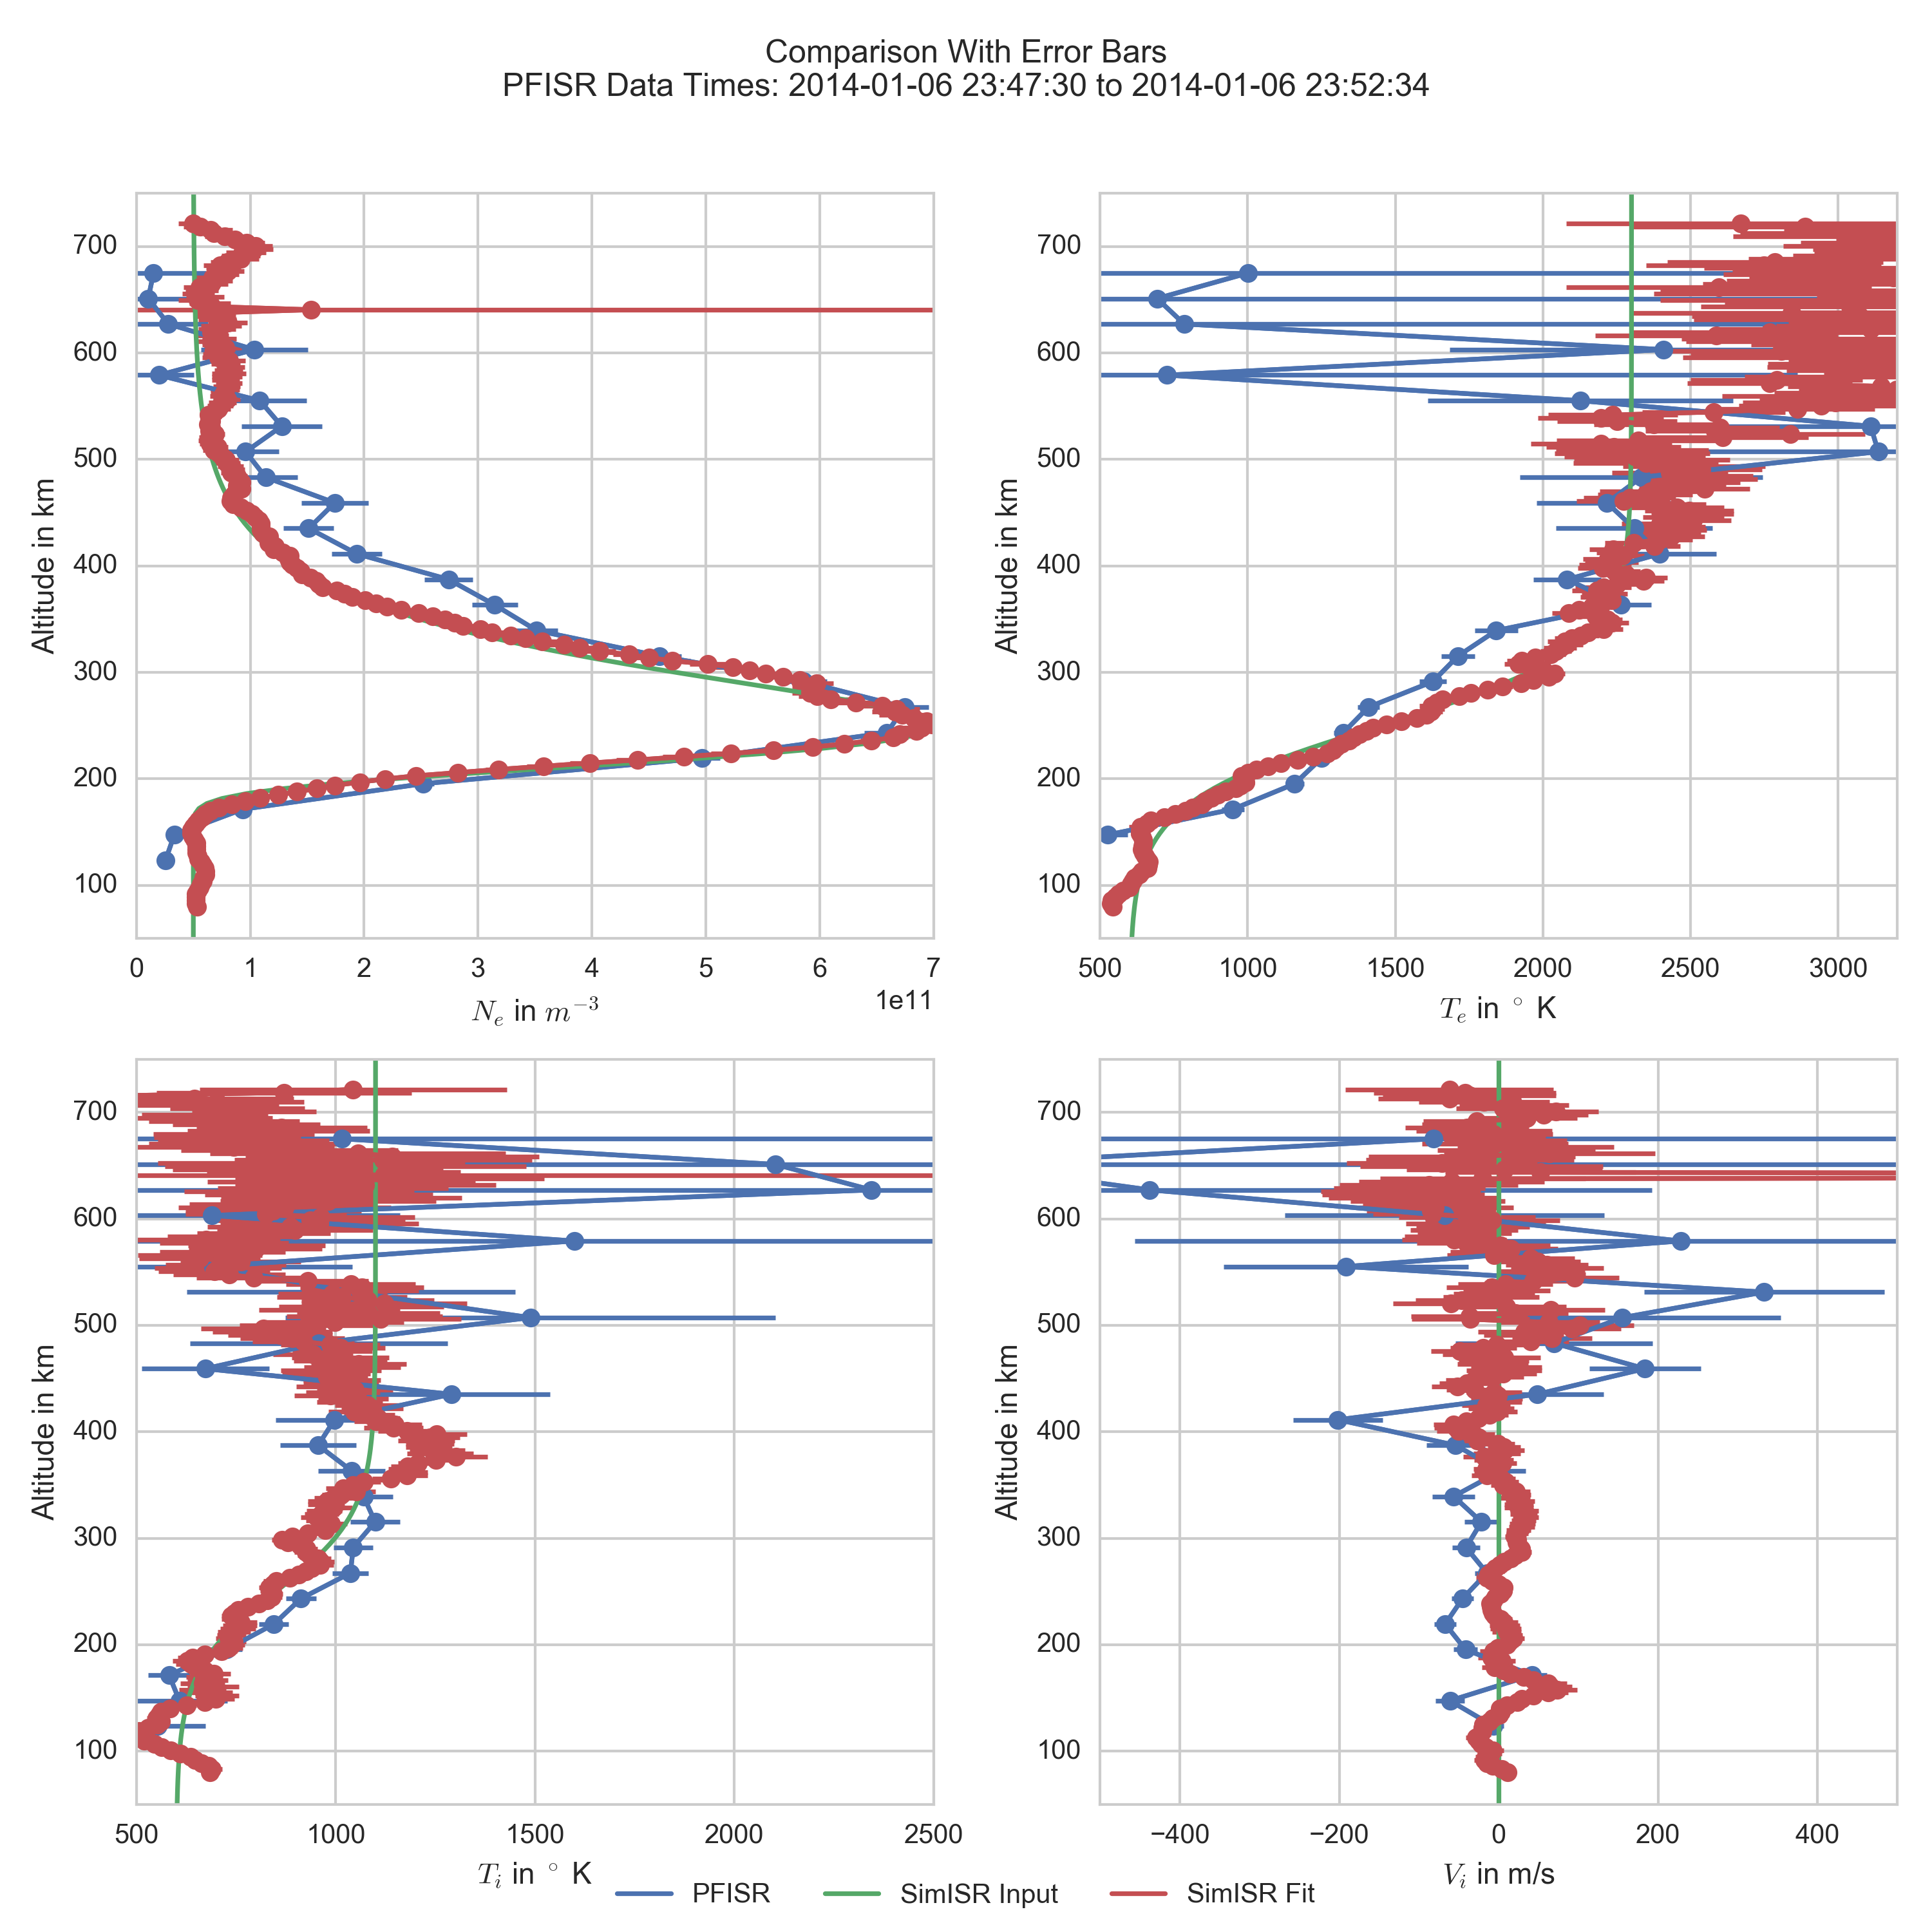
\includegraphics[width=4.5in]{Paramcompeb}
\caption{Comparison of real data from PFISR with SimISR data and a possible input parameter distribution along with error bars.}
\label{fig:simisrparamcompeb}
\end{figure}

Lastly a comparison of example ACFs and spectra are shown in Figure \ref{fig:simisrspectcom}. In both cases the ACFs were estimated using the method described in Section~\ref{section:isrproc}. This leads to a windowing of the ACF specified by Equation~\ref{eq:sumruleest}, and is the cause of the ringing artifacts seen in the spectra and that the $0^{th}$ lag is not the largest amplitude, as would be expected. Also of note is the lack of symmetry in the PFISR spectra, which is likely due to the mixing of different populations of plasma during the radar integration period of five minutes \citep{knudsen1993}. Still, qualitatively this shows relatively good correspondence between PFISR and SimISR and gives some confidence in the ability of SimISR to create realistic data. 

\begin{figure}[h!]
\centering
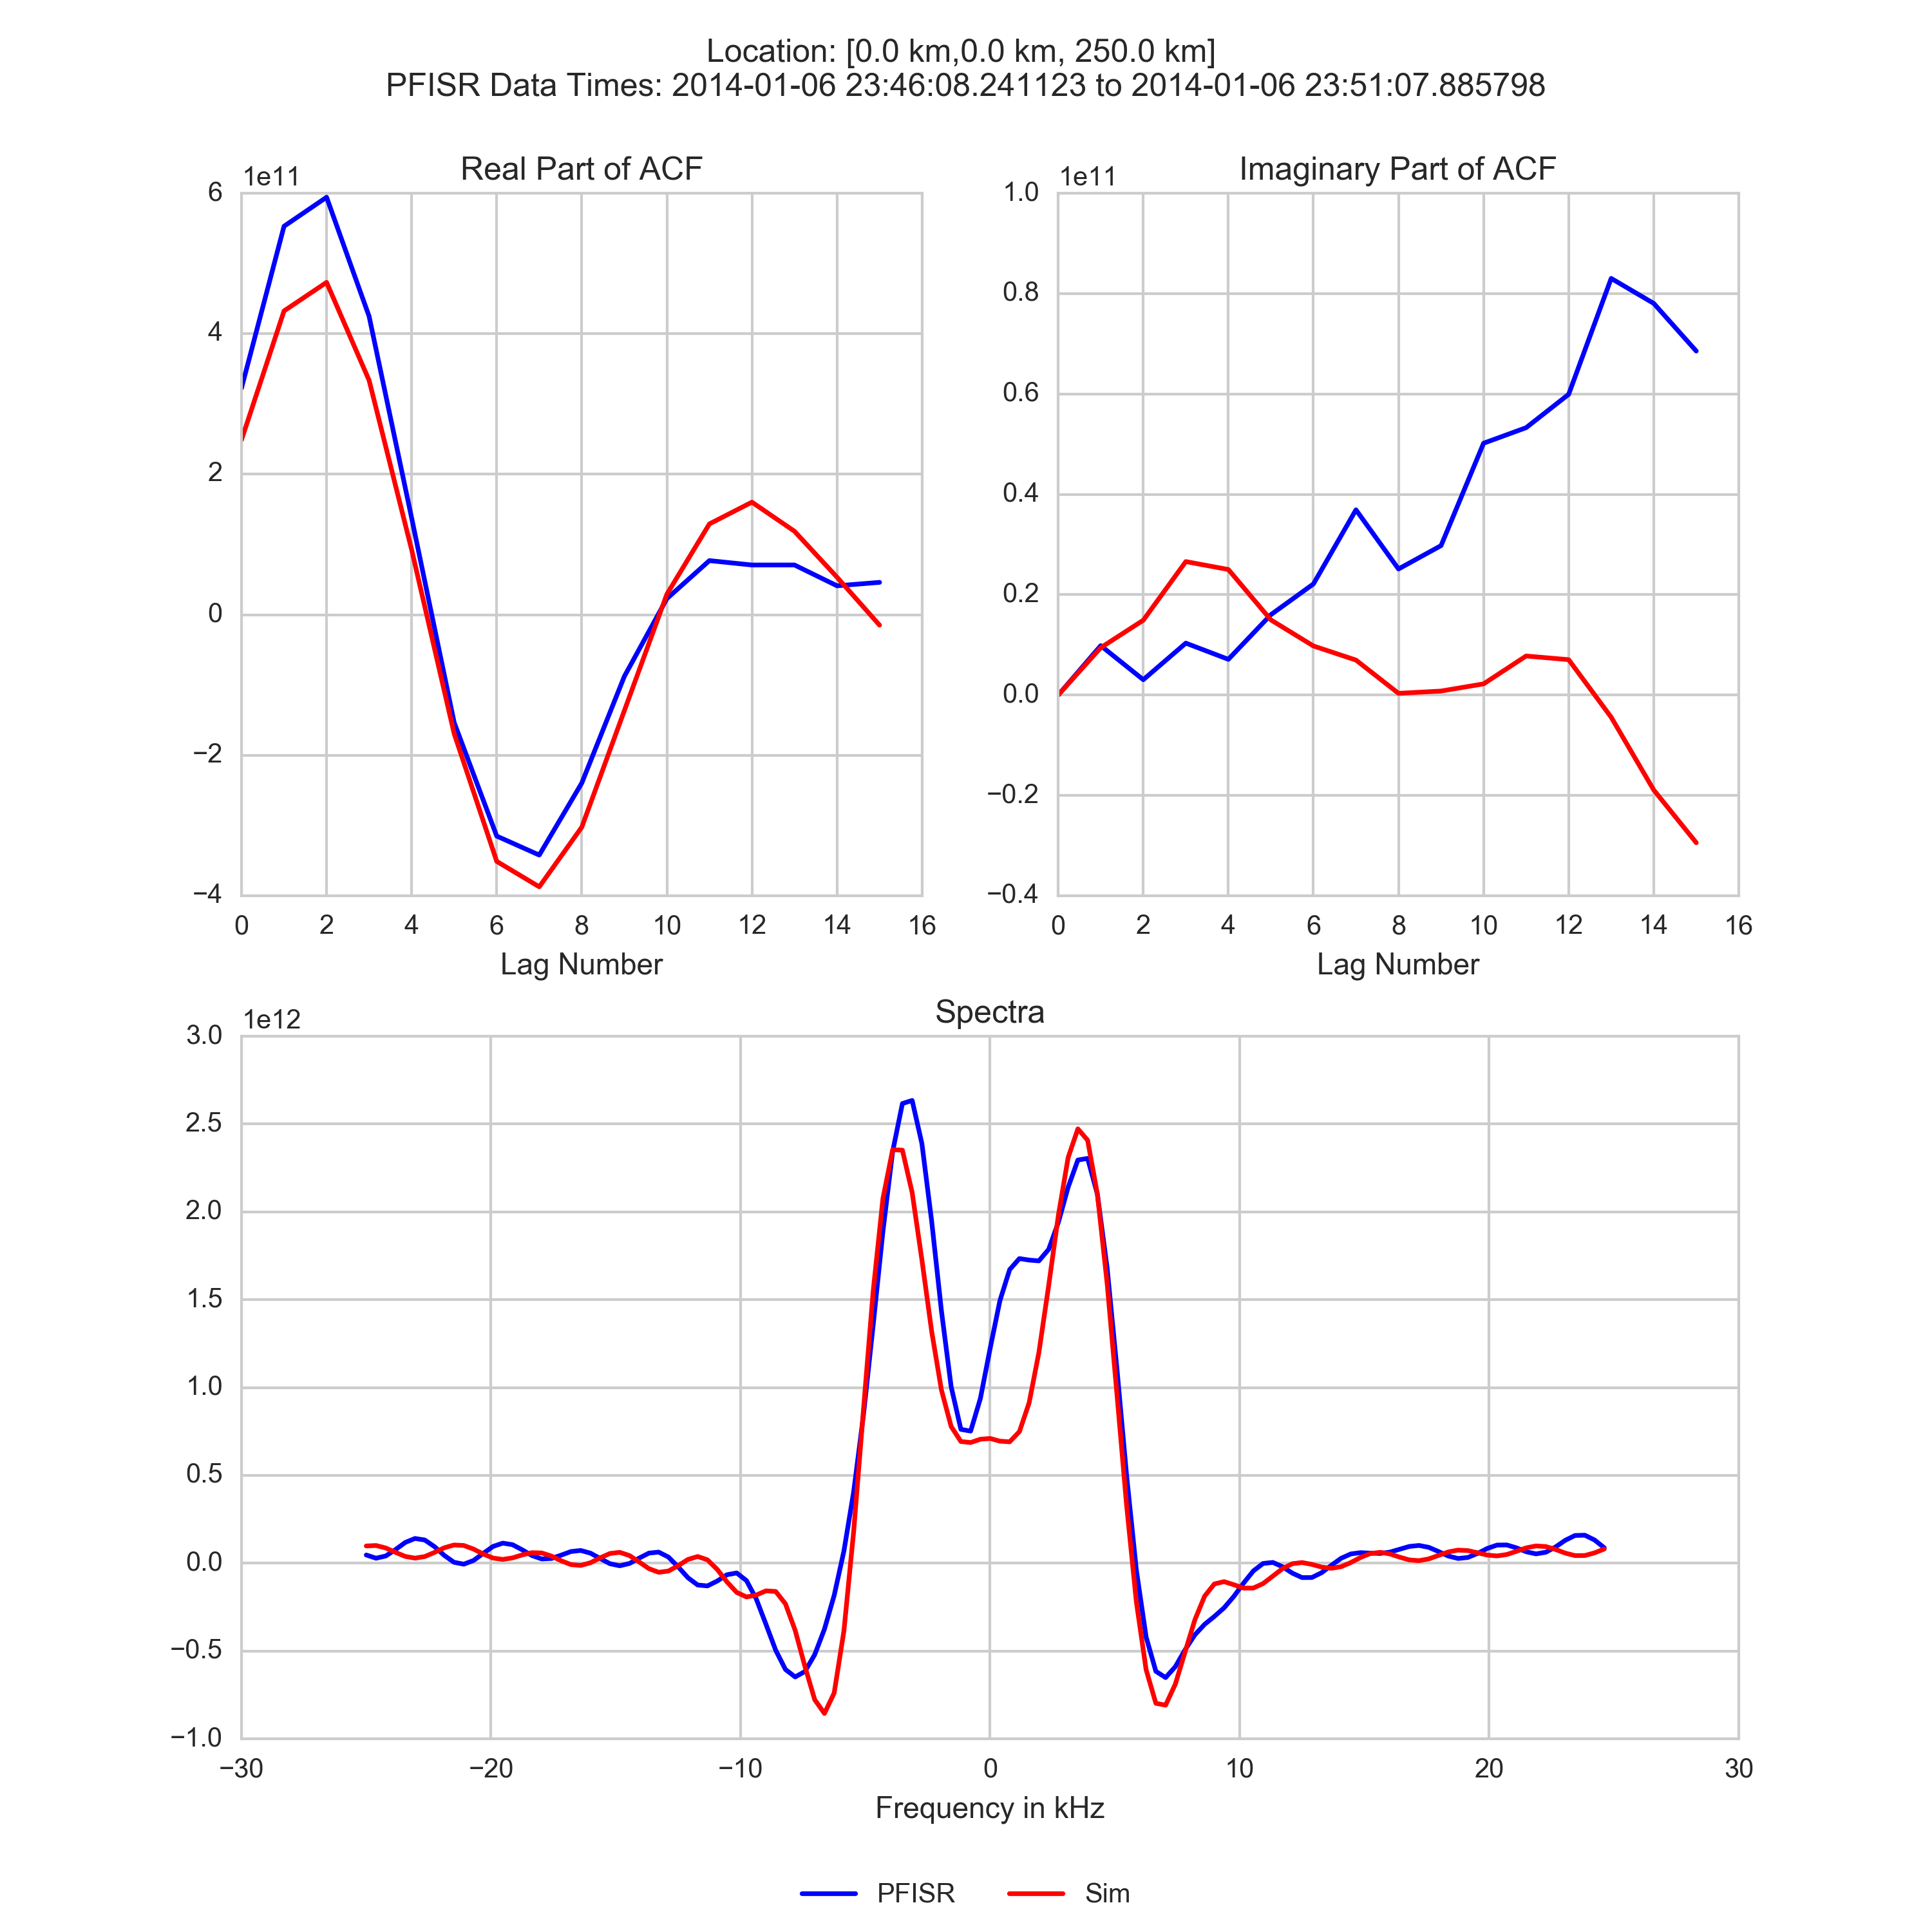
\includegraphics[width=4.5in]{speccomp}
\caption{Comparison of ACFs and spectra from PFISR with SimISR. In both cases the ACFs were estimated using the method described in Section~\ref{section:isrproc} thus adding a windowing function like in Equation~\ref{eq:sumruleest}.}
\label{fig:simisrspectcom}
\end{figure}

%\begin{figure}[!t]
%\centering
%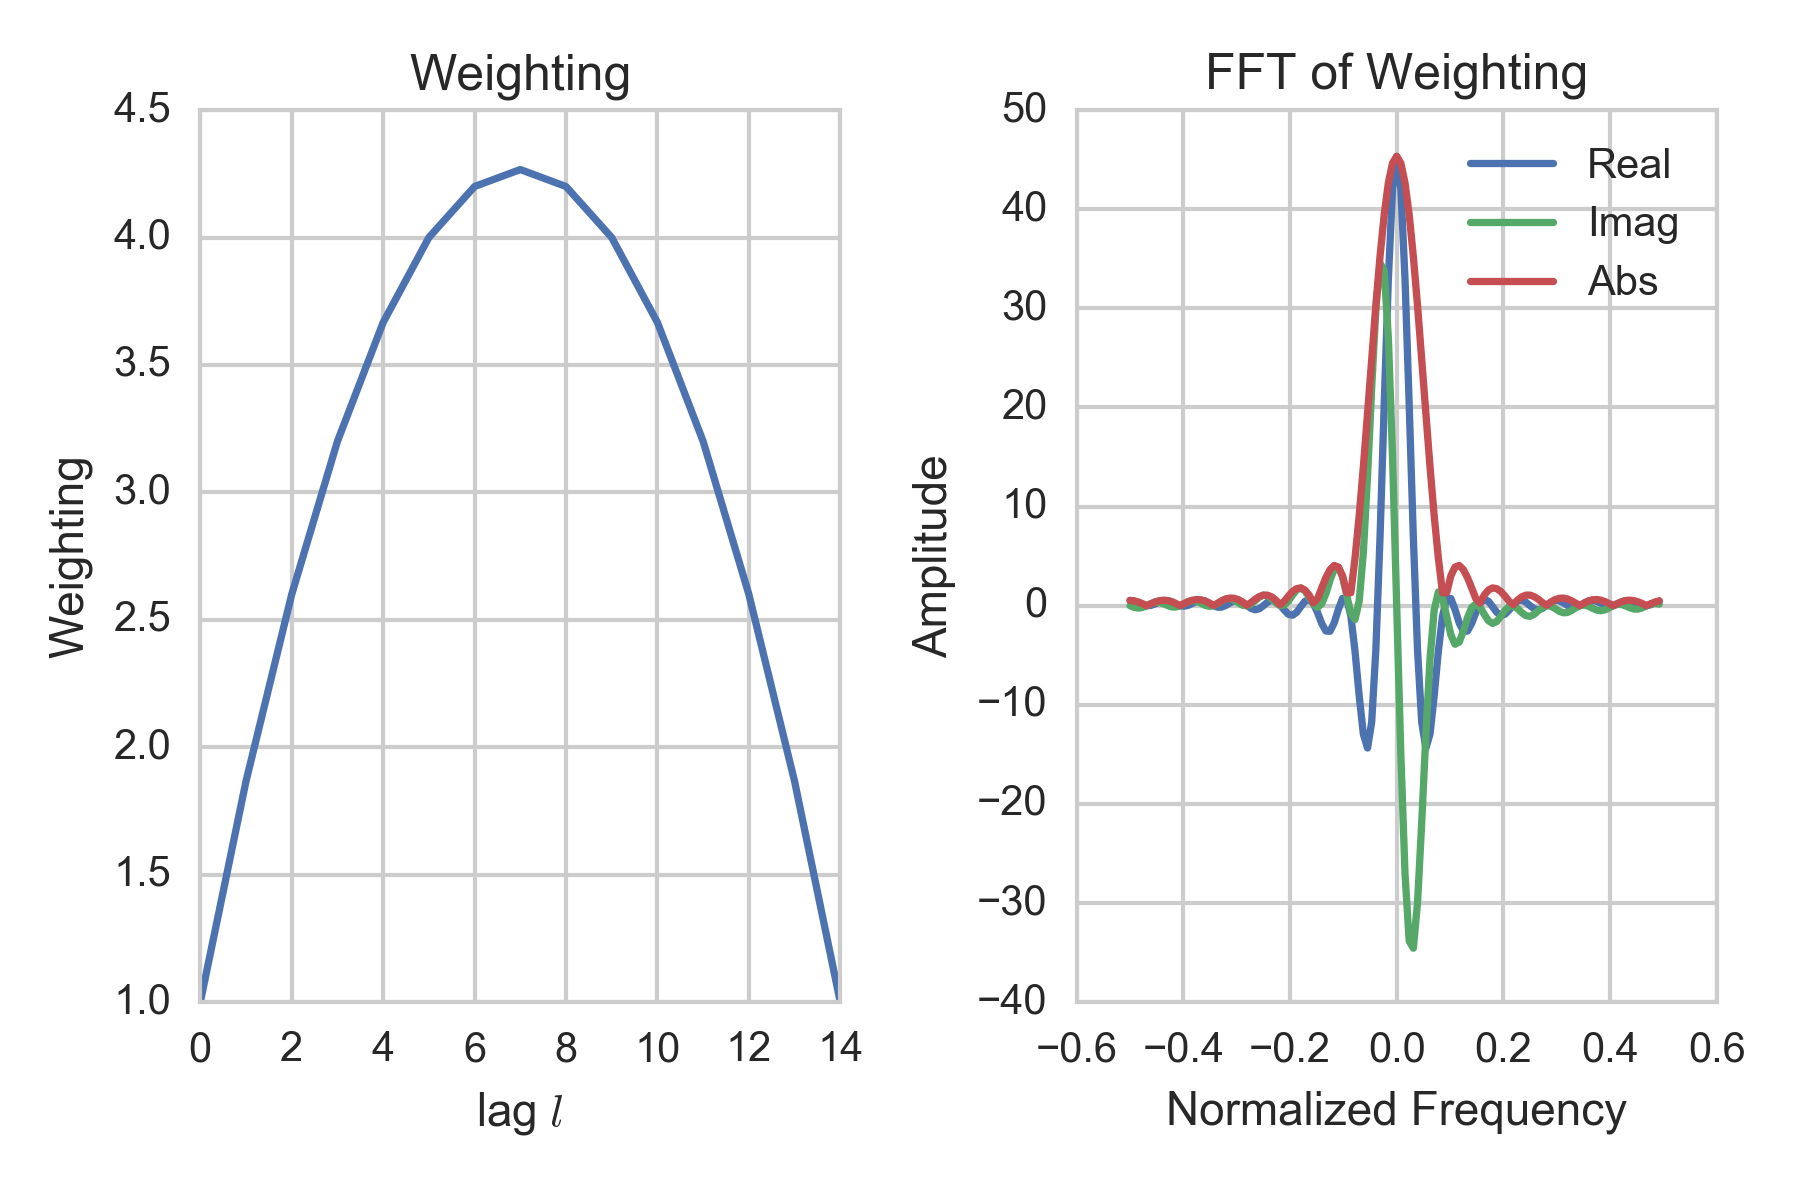
\includegraphics[width=6in]{ISRWindow}
%\caption{The window function that is applied to the ACF as seen in Equation~\ref{eq:sumruleest} in the left pane for $L=15$ and its 128 point length Fast Fourier Transform in the right panel. }
%\label{fig:isrwindow}
%\end{figure}

\subsection{Monte Carlo Example}

It is often necessary to obtain a large number of sensor measurements for a statistical study or for creating of a training data set for a pattern recognition algorithm. This can be a very burdensome search and classification task for the researcher if the input set must be drawn from actual sensor measurements. However, a number of useful cases exist where SimISR can be profitably employed to create a synthetic data set instead, saving considerable work over case assembly from a real ISR data based training set.  We explore one such example in this section.

% JOHN: you still need to work on this comment by Phil, no?   :
%\pcom{Very awkward and verbose; rewrite}{It is necessary to understand the statistics from the sensors used in scientific studies. In order to do this a large number of measurements must be taken with the sensor. There are issues with this approach in that the inputs can not be controlled so along with any random variation that may be found in the sensor the random variation of the measured process will be included and must be taken into account during the analysis of the data. With the simulator the statistical fluctuations from only the measurement mechanism only can be studied and thus reducing the uncertainty of the measurements.}
% Josh I updated the above paragraph to take care of Phil's comment. The point of the paragraph is I can make a training set instead of working through a data base to collect and classify data. Perhaps I can add a reference to pattern recognition book that talks about training sets.
For this example we show how distributions of plasma parameter measurements change as more pulses are averaged. To do this we created a field of constant plasma parameters typical of the high latitude ionosphere at around 250 km, and performed a Monte Carlo-type simulated statistical experiment using a number of independent realizations. We use the parameters for the PFISR system for this simulation along with the plasma parameter listed in Table \ref{tb:param1}. For a number of independent radar pulse counts, $J$, we used 4,600 realizations of the statistical ISR measurement process in each case to create statistical distributions of measured parameter values. To calculate distributions histograms are created using each of these relations, although some come from the same beam and thus there can be some statistical correlation. The distributions can be seen in Figure \ref{fig:statshistall} which show distributions where 200, 500 and 1000 pulses are used respectively. For a given pulse count $J$, the plasma parameters have a Gaussian-like distribution. As expected the distribution narrows as the number of pulses $J$ is increased. Another observation is that as the number of pulses increases the bias in the measurement is reduced, which could be due to the way that the histograms were calculated.
%% PJE:  However, Figure 5 clearly shows a biased measurement for the 200 pulse case slowly resolving to zero bias in the 500 and 1000 sample cases.  You need to address this behavior here, as a sharp reviewer is going to notice and call it out.  I don't offhand know why that is happening.
%% JPS: Didn't have a great answer, I have a feeling that it might be related to how I calculated the histograms. I took data from all of the beams together so there correlations between some samples. The  
%% PJE: I guess then you need to leave it alone, but I would be prepared for questions.
%% JLS:  So it doesn’t actually resolve to 0, at least in the density histogram.  For large number of pulses there seems to be a second bump at 0.7e11.   Would it be worth looking at some ACF fits for those cases to try and see if there is some obvious explanation?  Are you adding receiver/sky noise for these runs?   Could incorrect noise subtraction, or maybe some coloring in the noise generation, be a cause?  I’m confident that a reviewer will raise this issue, so best to just get our response together now!
\begin{table}[!t]
\centering
\caption{Simulation parameters.}
\label{tb:param1}
\begin{tabular}{ll}
Species & O+ e-\\
$N_e$    & $1\times 10^{11}$ \\
$T_e$      & $2100^\circ$ K   \\
$T_i$      & $1100^\circ$ K \\
$V_i$      & $0$ m/s
\end{tabular}
\end{table}

\begin{figure}[!t]
\centering
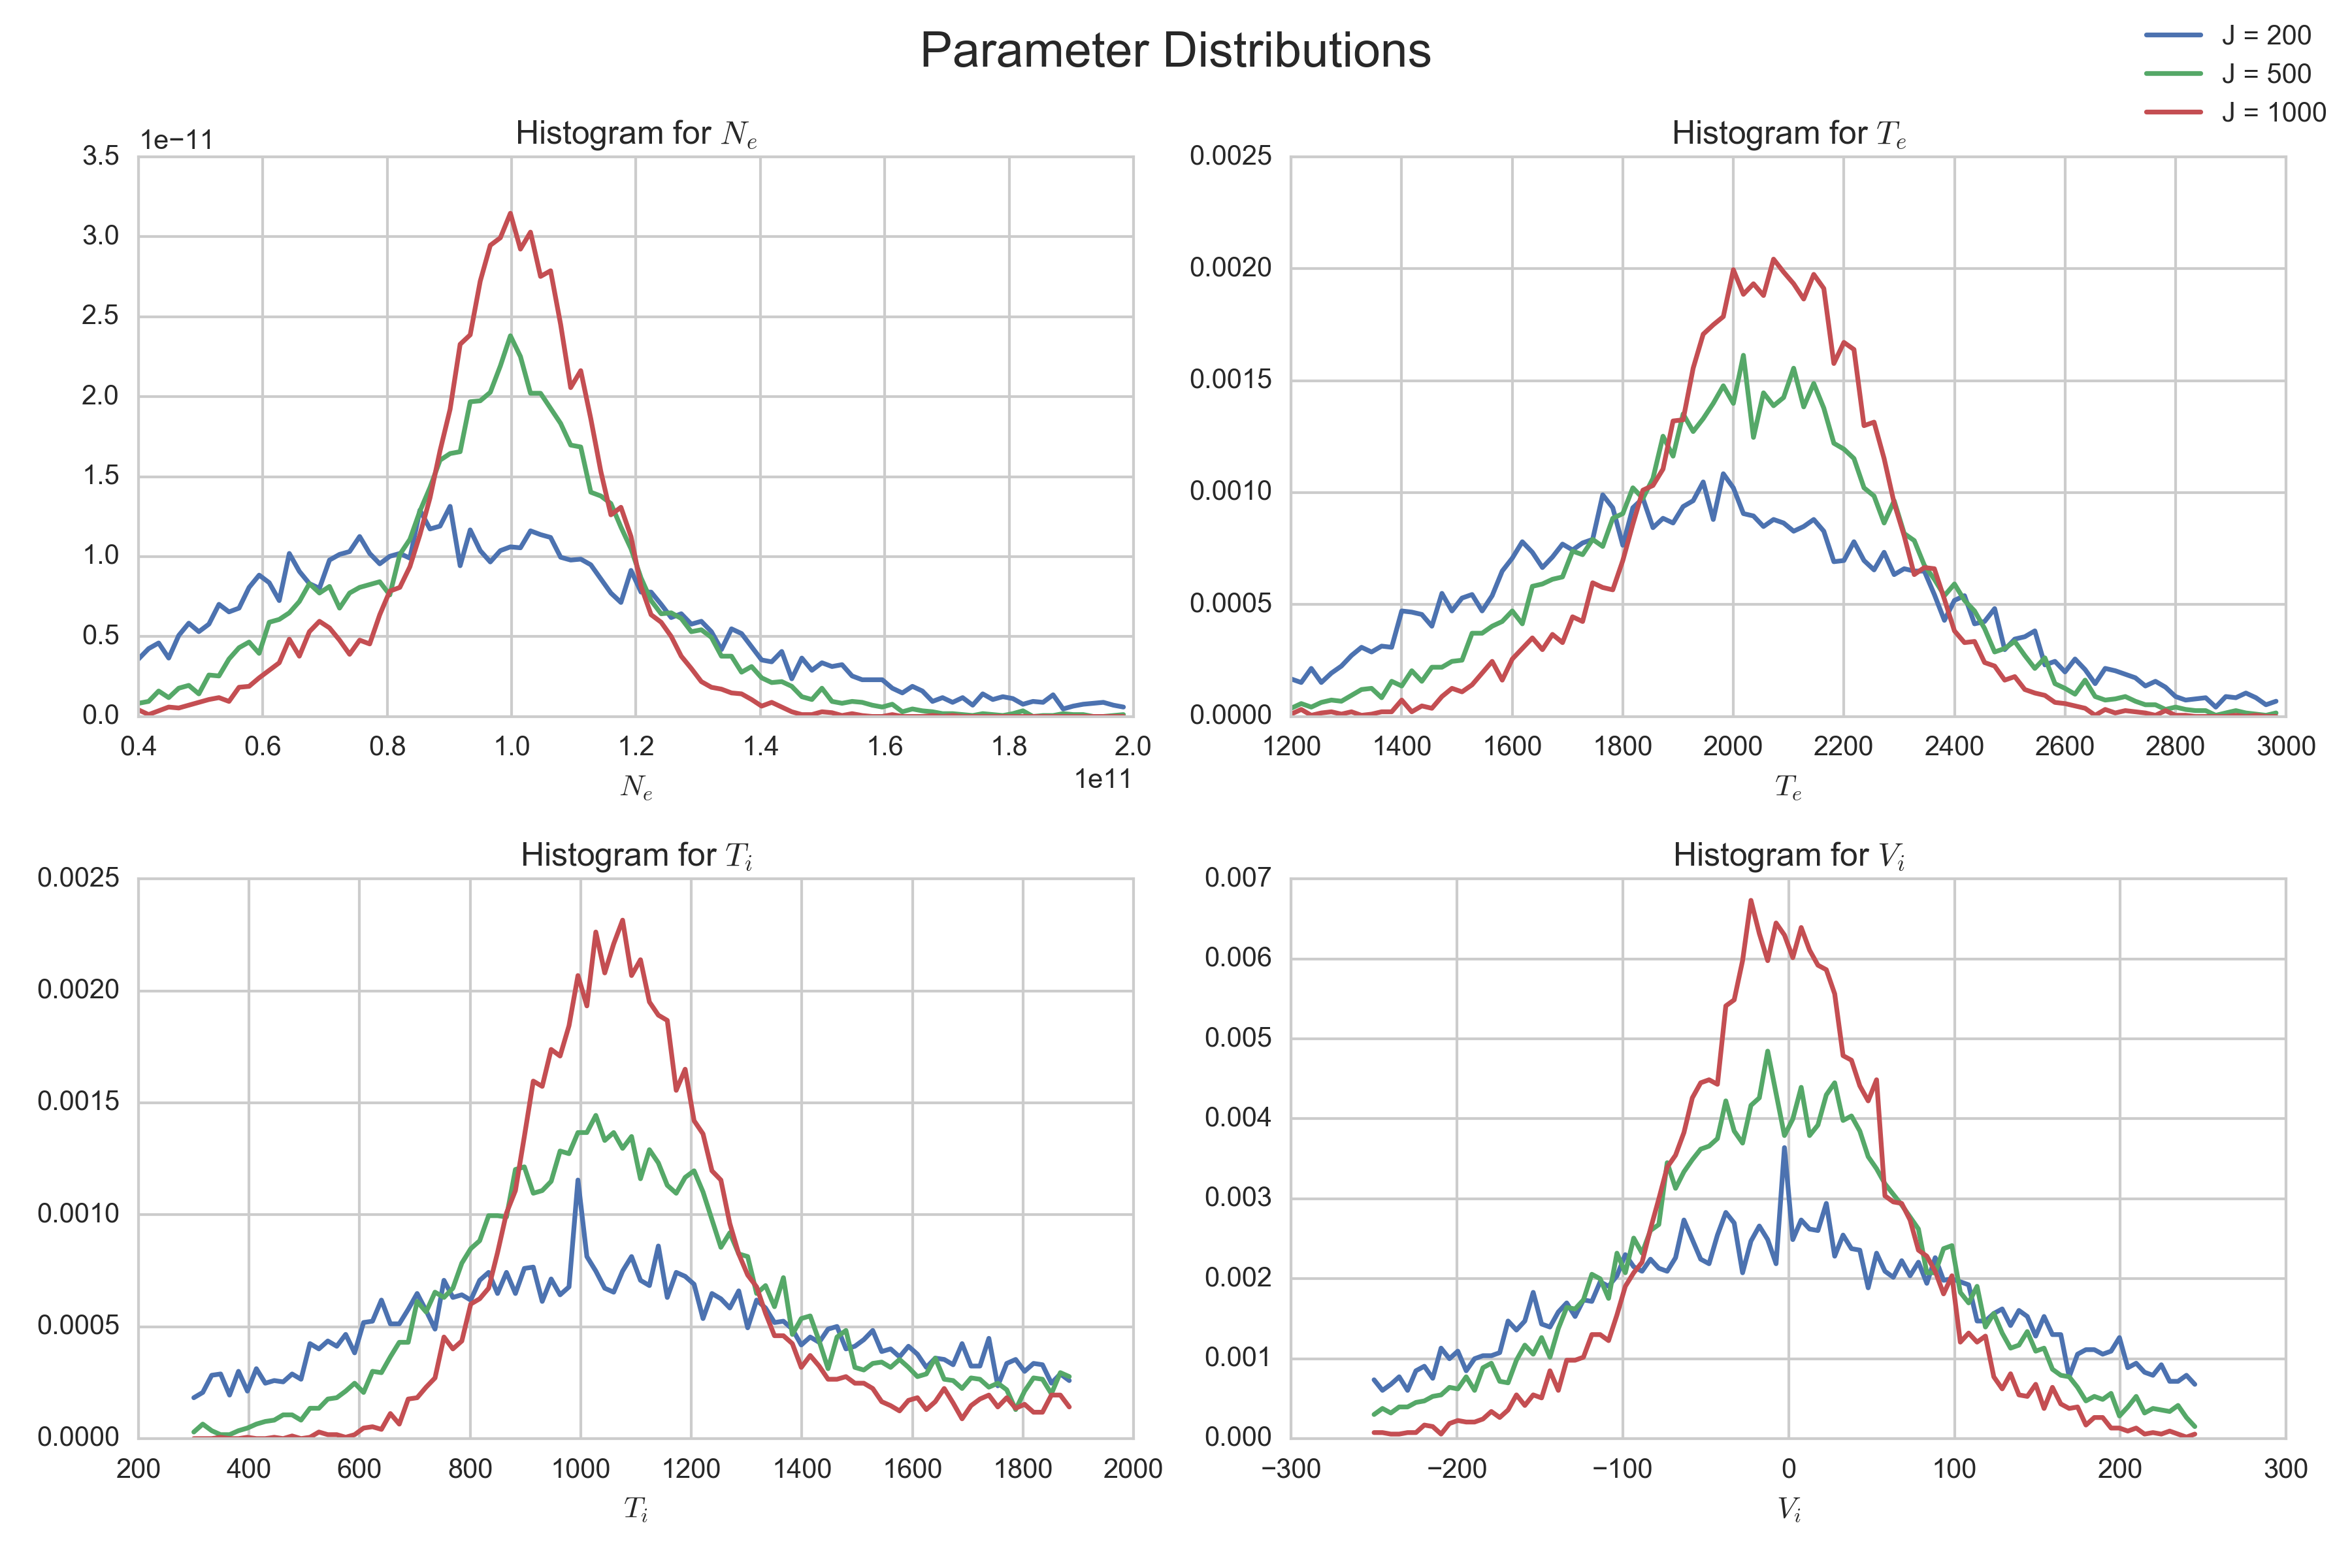
\includegraphics[width=5in]{datahist}
\caption{Normalized histograms of fitted plasma measurements from cases with 200, 500 and 1000 pulses integrated. These are estimates of probability density functions for each of the plasma parameters measurements given the values in Table \ref{tb:param1}.}
\label{fig:statshistall}
\end{figure}

ISR error analysis also benefits from SimISR's ability to generate a large number of samples of fitted parameters. In particiular, ISR measurements need to have estimates of the errors, and accuracy of the estimates of these errors can be explored using SimISR. Using the 1000 pulse case seen in Figure \ref{fig:statshistall}, we can compare simulated output distributions with the actual distribution of parameter values. Figure \ref{fig:statshistsingle} shows a comparison of these two different models using. The first method, represented by the blue line, uses the sample mean and variance calculated from each as the variance and mean for a Normal distribution. The other method, which generated the green line, calculates an average squared error from the true value for each parameter for the variance in a Normal distribution and uses the true value for the mean. 
%% PJE: I'm confused by the logic of this sentence above (also "shows gives" etc?) - please reword.
%% JPS: Just changed 
This example shows that the parameter distributions are well represented by a Gaussian function but that the error estimated from the fit may not give a completely accurate representation of variance of these parameters. 

\begin{figure}[!t]
\centering
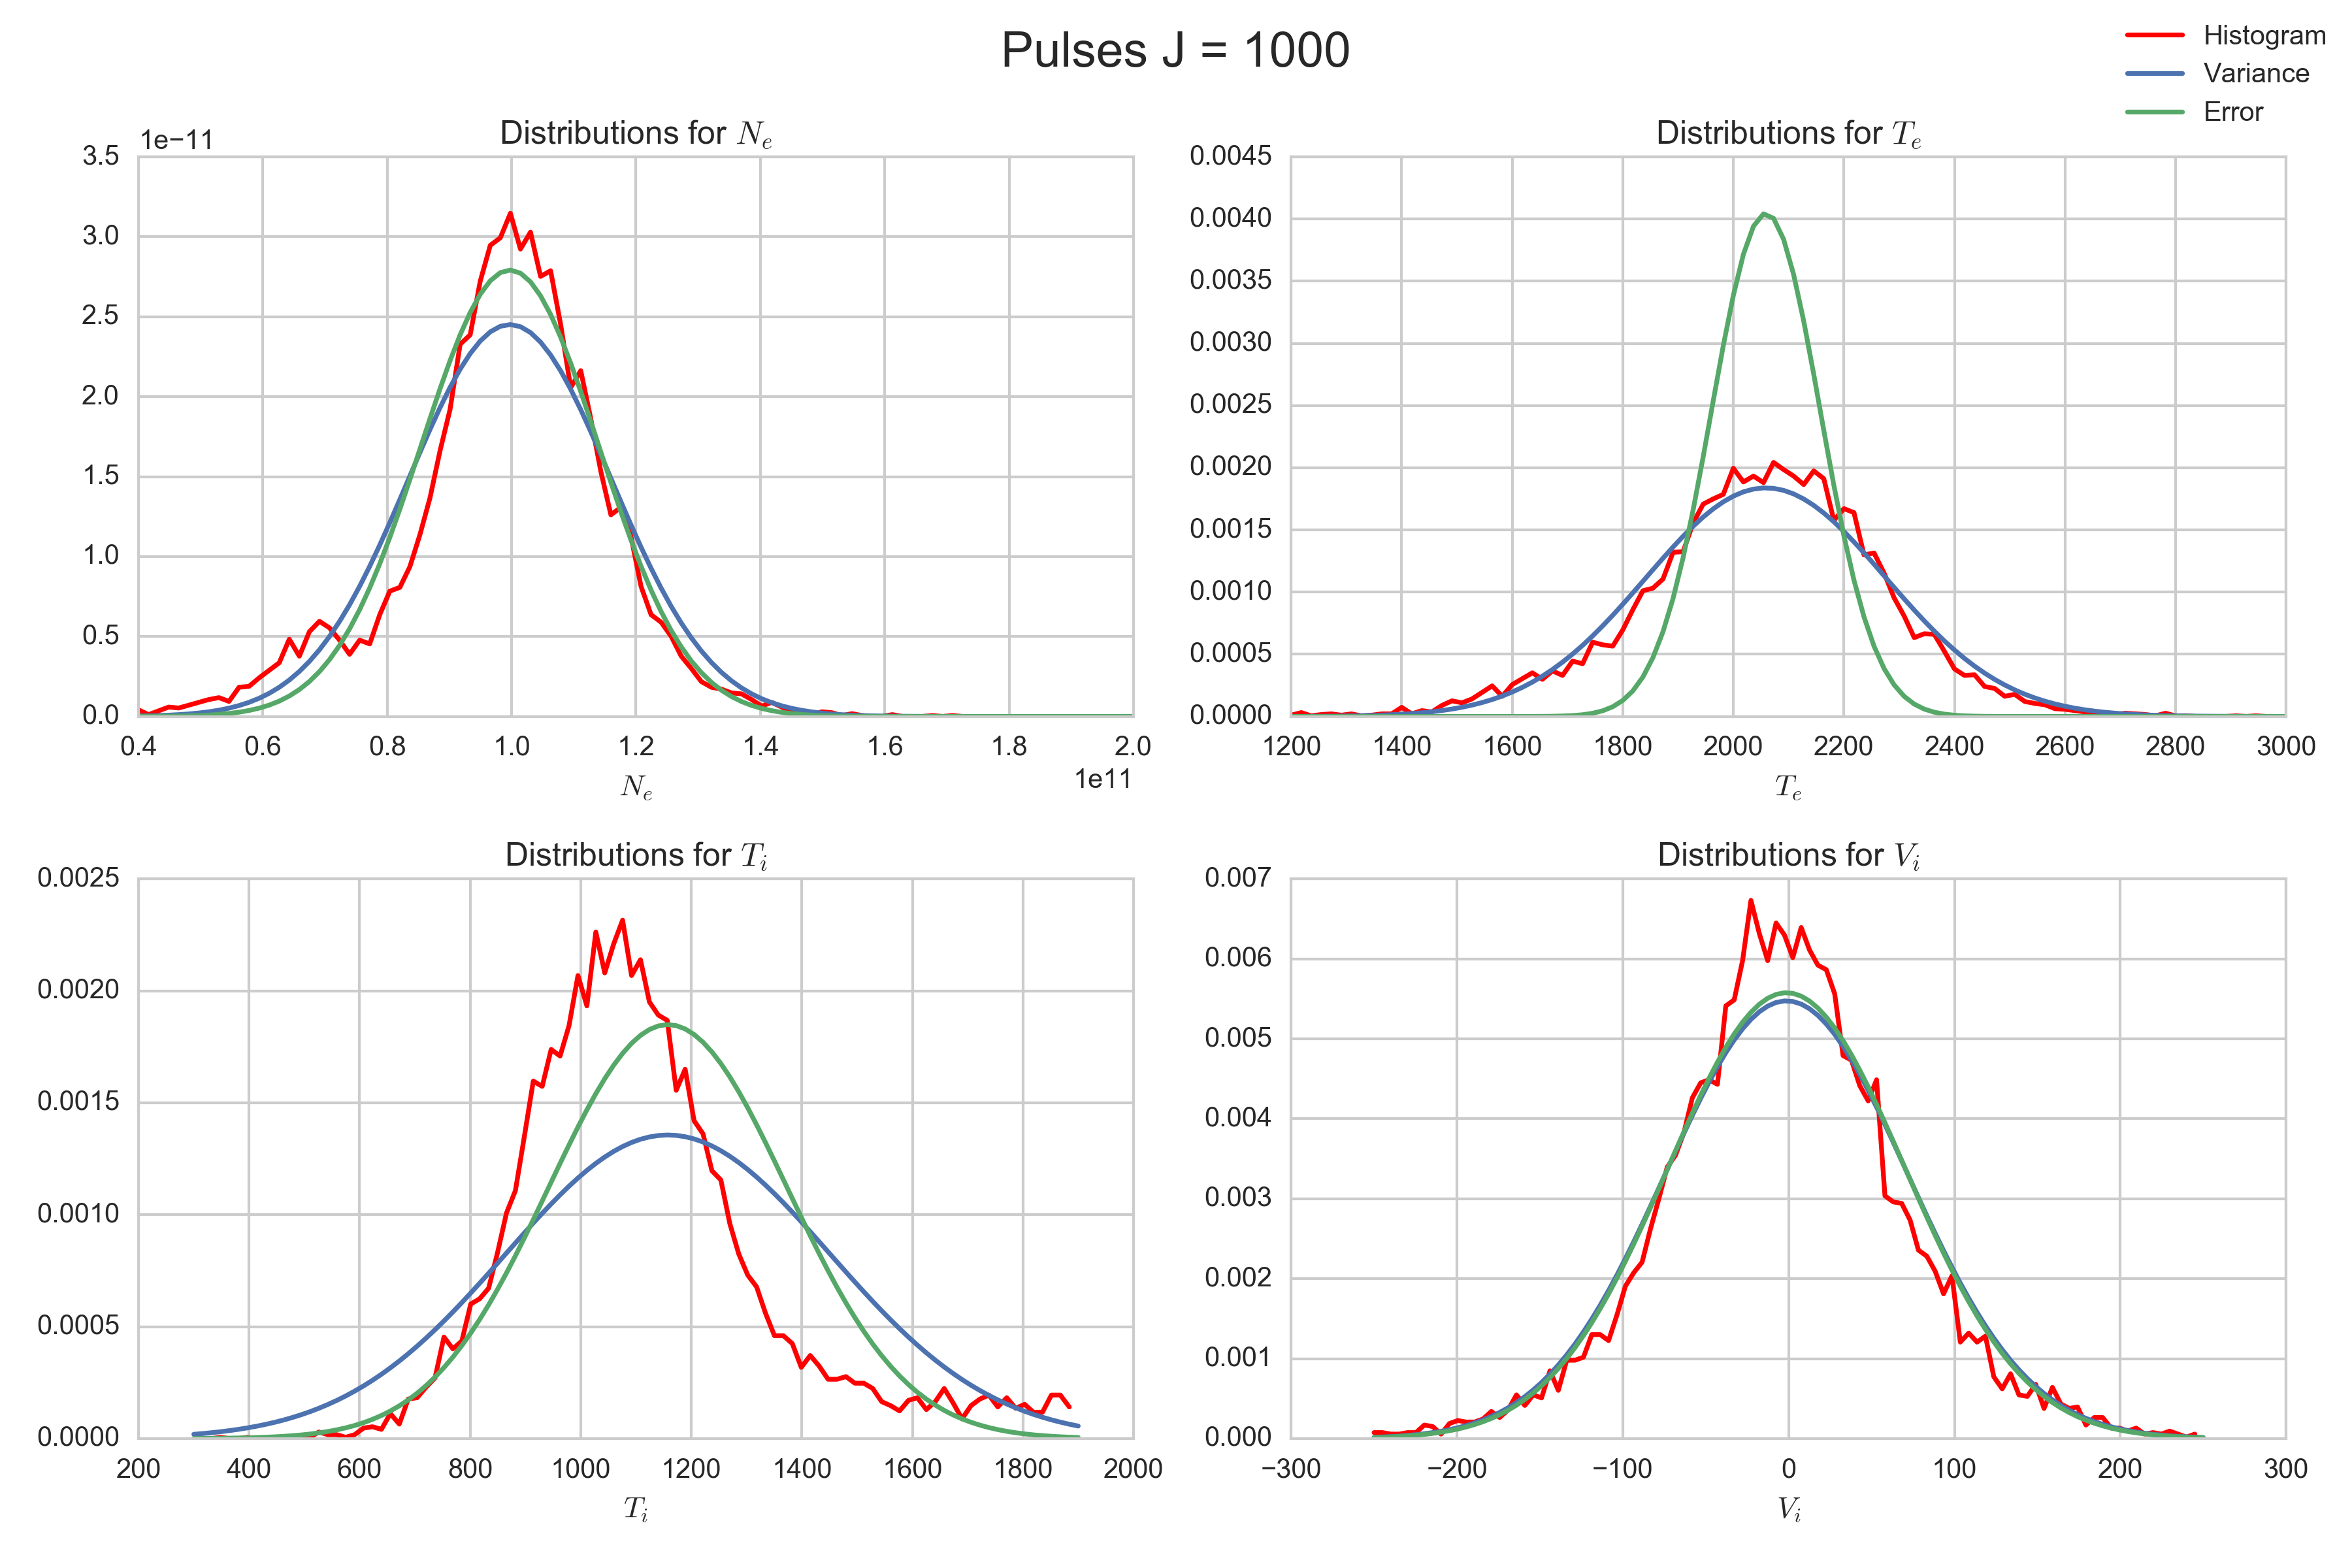
\includegraphics[width=5in]{histsingle}
\caption{Distributions of fitted plasma measurements from cases with 1000 pulses integrated. The red curve shows the actual distribution derived from a histogram of 4600 measurements. The blue curve is a Normal distribution using the MSE from the measurements as the variance and the average parameter value as the mean.  The green curve is a Normal distribution using the average estimate of error squared that comes with the parameter measurement as the variance and the average parameter value as the mean.}
\label{fig:statshistsingle}
\end{figure}


The SimISR tool is useful for identifying situations where assumptions in the parameter fitting break down. For example, a number of studies have explored the case where ISR parameter measurements and spectra show evidence of non-Maxwellian plasma behavior (for AMISR examples see \citet{Akbari:2012dz,Akbari:2015fv}). Future studies using the simulator could help create a training set that can be used with a pattern recognition algorithm to identify cases where normal fitting procedures may be incorrect due to violation of Maxwellian assumptions.

\subsection{Electron Density Measurement}
An important aspect of experiment design is determining the observability of plasma phenomena with ISR. The simulator can be used to help understand the trade space accompanying a given experimental configuration. With this in mind, we use a simple two dimensional spatial field of ionospheric parameters as an illustrative case study. An all-O$^+$ ionosphere is created with a background electron density that follows a Chapman function with $1\times10^{11}$ m$^{-3}$ as the peak value and a constant electron and ion temperatures of 2000 K and 1500 K respectively. The background ionosphere is depicted in Figure \ref{fig:backgroundnsamp}.

\begin{figure}[!t]
\centering
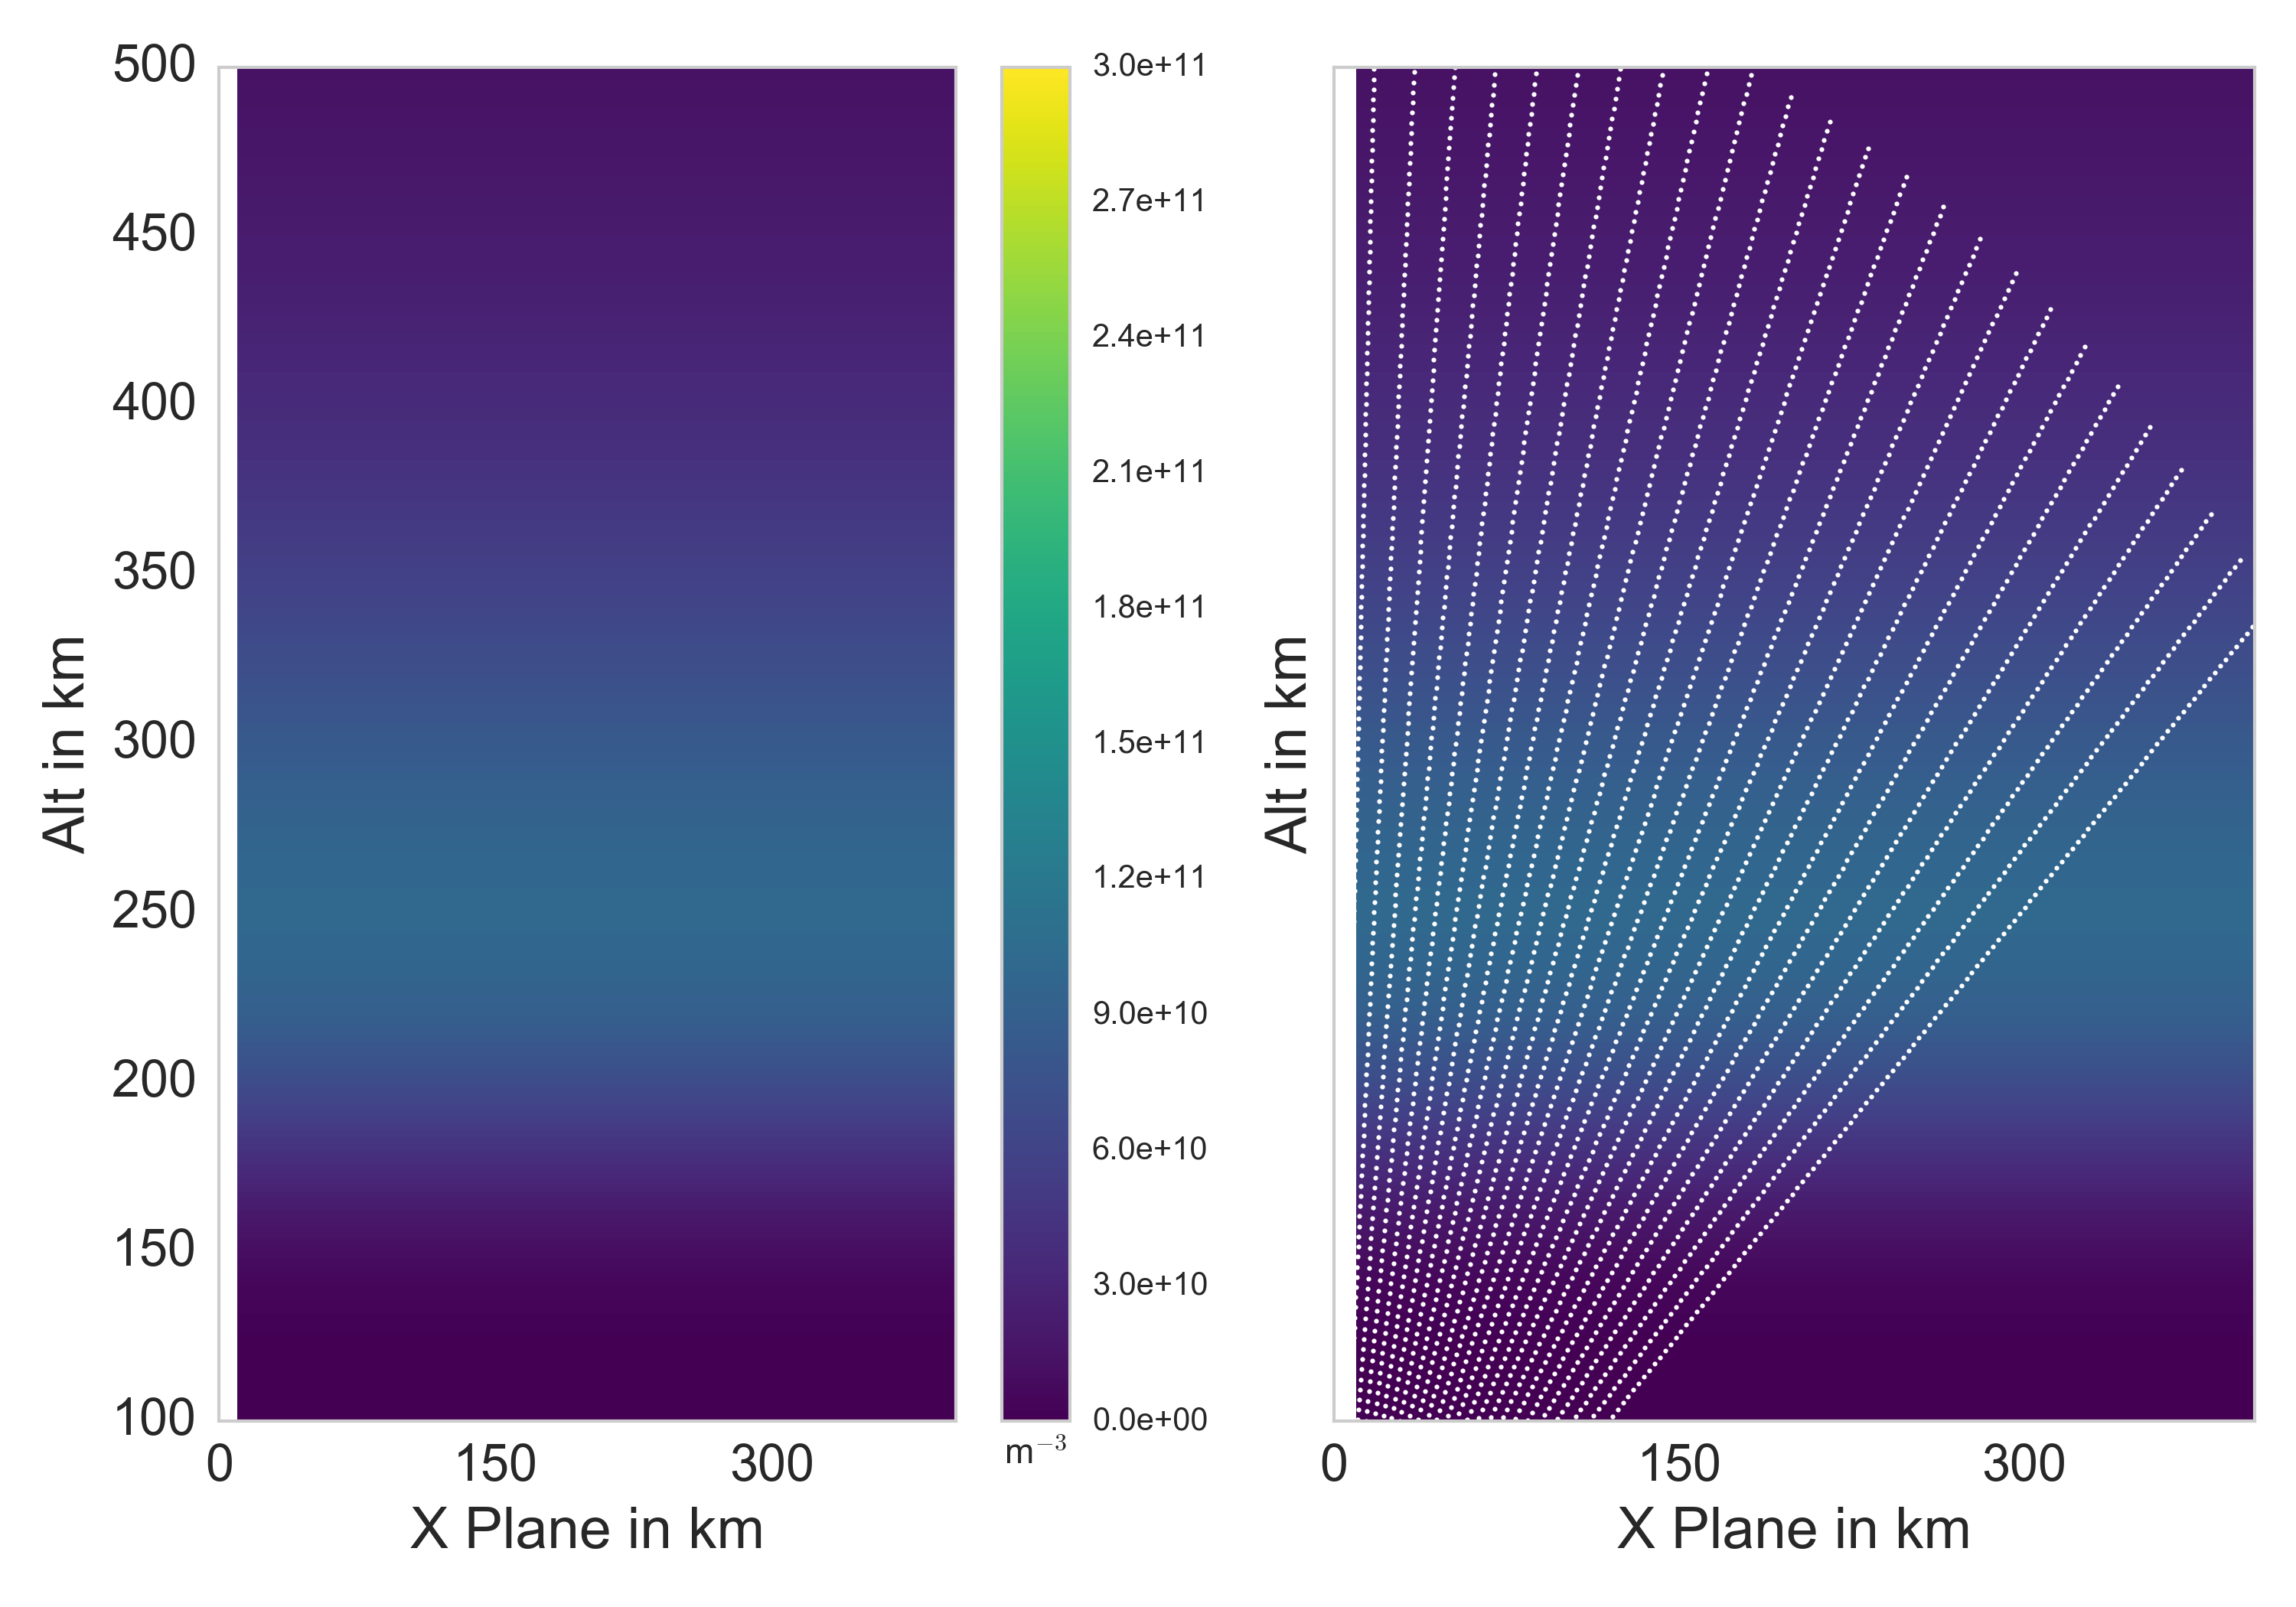
\includegraphics[width=3.5in]{backgroundandsamp}
\caption{Contour of background $N_e$ for simulations and the spatial sampling pattern overlayed as white dots.}
% JOHN:  you don't need both of these panels, just the one on the right along with the colorbar.   Also, you should reduce the number of labels on colorbar, increase the font, and absorb exponent into units (which are not given).  Also there is no indication of what scalar is being plotted.   Typically you would write parameter/units above the colorbar:   $N_e (10^{10}$m$^{-3})$.   This comment goes for other plots too.
% Josh: I've updated the figures as you suggested.
% MZ - why run the colorbar out to 30 instead of the max density (~1.5e11) for this field?  Maybe because you want to keep the same colorbar for all density plots?
\label{fig:backgroundnsamp}
\end{figure}

%For these simulations we want to show how ambiguities could arise when trying to image just simple electron density enhancements with the beam pattern shown in the right panel of Figure \ref{fig:backgroundnsamp},
We first explore how a thin stationary density enhancement is resolved with the radar beam pattern shown in Figure \ref{fig:backgroundnsamp}, where each dot is a range gate in one of the 25 beams used. In Figure~\ref{fig:stationaryall}a, a thin density enhancement 2 km in width and 5 times the background is placed in the radar field of view. The enhancement is at the resolution limit of the original Cartesian grid, a delta function in the x direction.  The fitted electron density results from our simulation, without any additional averaging beyond the processing described in Section \ref{section:isrproc},
%JOHN:  I don't know what "results of a single realization of our simulation" means here.  Is this different than "results of our simulation"?
%Josh: No extra averaging of fitted parameters.
are seen in Figure \ref{fig:stationaryall}b and \ref{fig:stationaryall}c using 15 and 60 second integration times, corresponding to 60 and 240 pulses per position, respectively. The different integration times show that, although the enhancement is blurred, the variance of the measurement impacts the quality of the reconstruction because of the inherent noise-like nature of of the signal. The expected errors for both of the reconstructions are shown in Figure \ref{fig:errorstationaryall}. As expected, the estimated errors show that uncertainties are larger for the case with fewer pulses (i.e. smaller ensemble average size). 
%JOHN:  I've tried to fix figure referencing in the above since it didn't mesh with what you had.   Also, how are you deriving density, is it just range corrected power here, or full spectrum fitting?  
%Josh: Fitted density, I mention it in the previous paragraph
Because we know the input parameters, we can do a quick comparison using the root mean squared error (RMSE) for each case. By comparing the RMSE between the 15 and 60 second integration cases, we find that the ratio between the two cases is approximately 5.4 in the simulation output.  However, the expected RMSE ratio between the two should be approximately 2 since the variance of the ACFs scales as $1/\sqrt{J}$, where $J$ is the number of pulses. If we instead use a median instead of a mean operator in the error calculation, this ratio becomes 1.55, more in line with the expected statistical error scaling, largely due to the large outliers being disregarded.  Further investigation of the quantitative error discrepancy is a larger effort and beyond the scope of this study.  However, in general, the ratios between the errors and expected errors are relatively close when employing a median estimator that inherently rejects large outliers.
%% PJE: You've left me hanging here though - what does this result mean?  It deserves at least one sentence worth of comment.
%% JPS: Commented further, the behavior of the expected errors and actual errors are relatively close
\begin{figure}[!t]
\centering
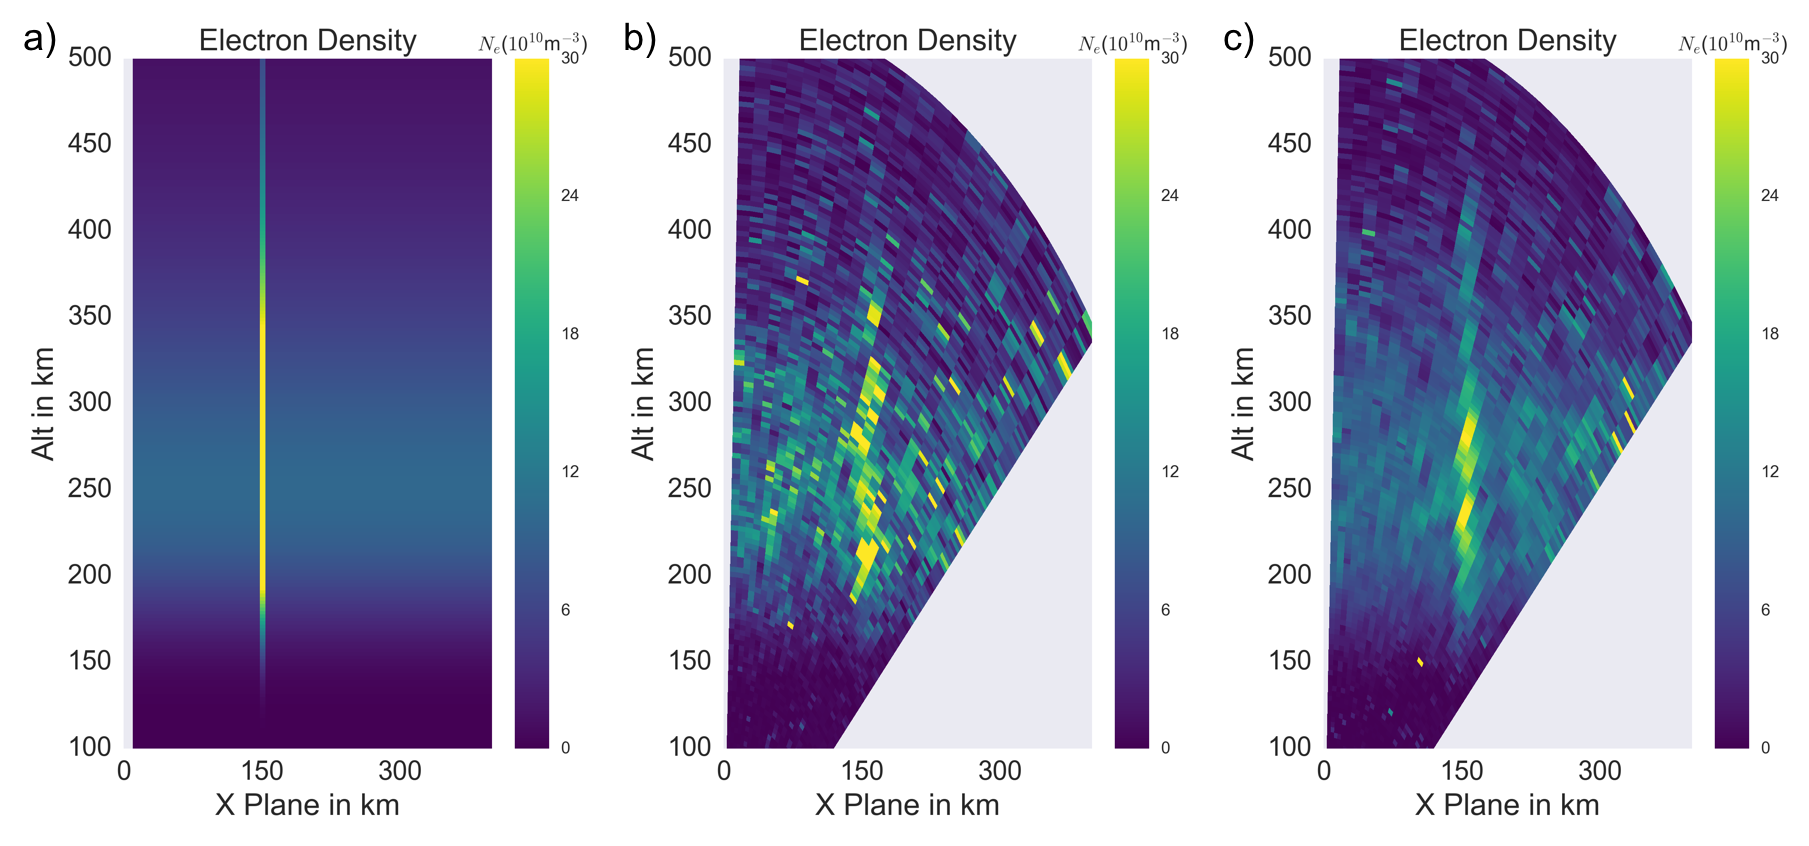
\includegraphics[width=6in]{stationary}
\caption{Results of stationary enhancement simulation. a) Input $N_e$. b) Output of simulator with 15 second integration. c) Output of simulator with 60 second integration.}
\label{fig:stationaryall}
\end{figure}

\begin{figure}[!t]
\centering
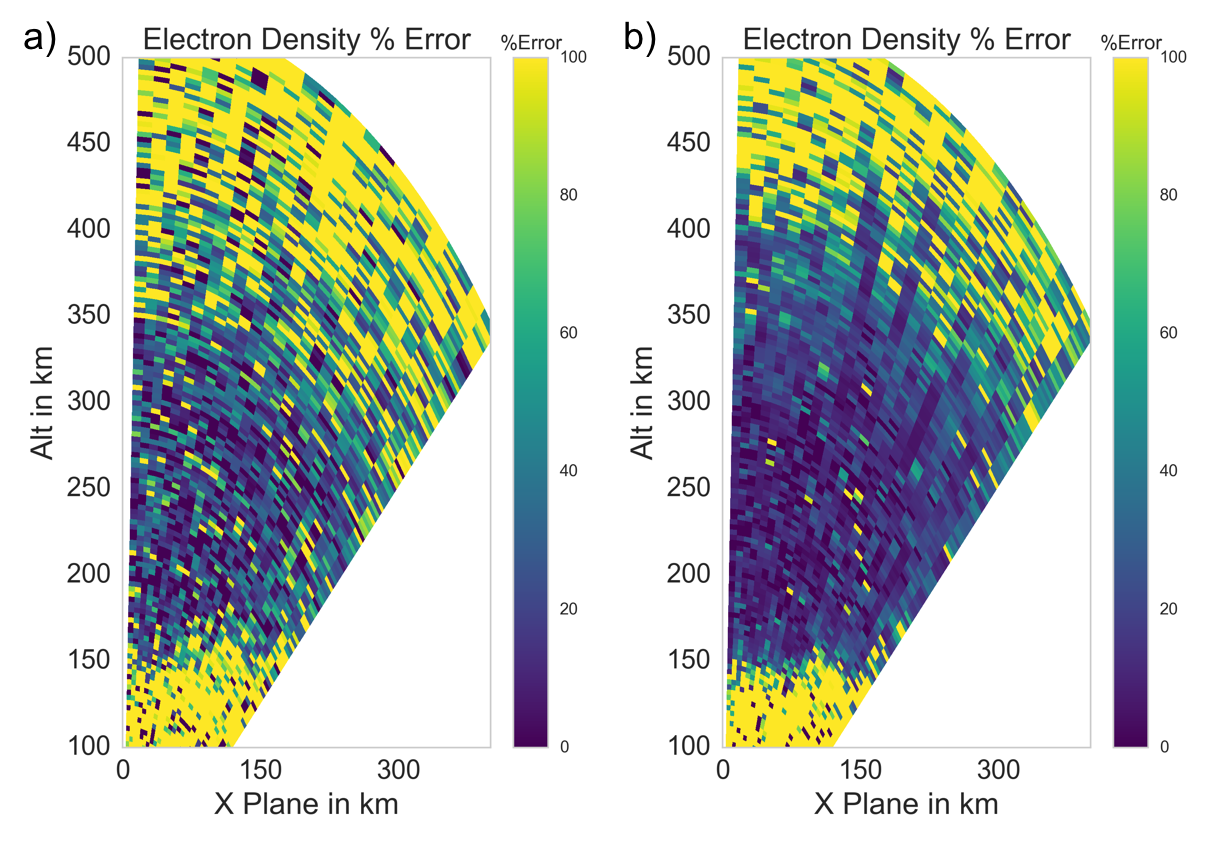
\includegraphics[width=4in]{Errorstationary}
\caption{Standard deviations from Figure \ref{fig:stationaryall}. a)  Estimate from fit for 15 second integration example. b) Estimate from fit for 60 second integration example.}
\label{fig:errorstationaryall}
\end{figure}

The blurring effect seen in this case study is not constant throughout the simulated space due to the way the radar samples the space. This is illustrated in Figures \ref{fig:moving10mins} and \ref{fig:moving14mins}, where as the enhancement moves through the scene at 500 m/s, its apparent size is affected by the orientation of the radar beams. 
%% PJE: please state the motion speed used
%% JPS: Done
As the enhancement becomes parallel to the radar beams, close to 0 km in the X plane,
%% PJE: where does it become parallel?  I cannot see the effect you are talking about here without some circles or arrows or something on the plot.
%% JPS: Done
%% JLS:  Actually the effect is more nuanced than just becoming thinner.   The density column is bifurcated below 200 km (two columns with gap in between).   DO you know why this is?  Is it a consequence of the shape of the ambiguity function, such that the target "fades" as it moves across beams?
its morphology in the reconstruction becomes smaller along the X-axis, as the range ambiguity is much larger than the cross range ambiguity. In both cases the expected errors, shown in panel c in both Figures \ref{fig:moving10mins} and \ref{fig:moving14mins}, give us confidence in these results as they are much lower value than the enhancements and background.
%% PJE: the electron density error plots here have the wrong scaling - everything is very dark color and I can't see any structure in any of them.  Please rescale the color bars.
%% JPS: added statement about errors
%% JLS: Hard to read the scales, but looks like you are using the same range for data and error.  The saturated error pixels don't matter, so why not compress the range so reader can visualize error in vicinity of the features we are trying to reconstruct?
\begin{figure}[!t]
\centering
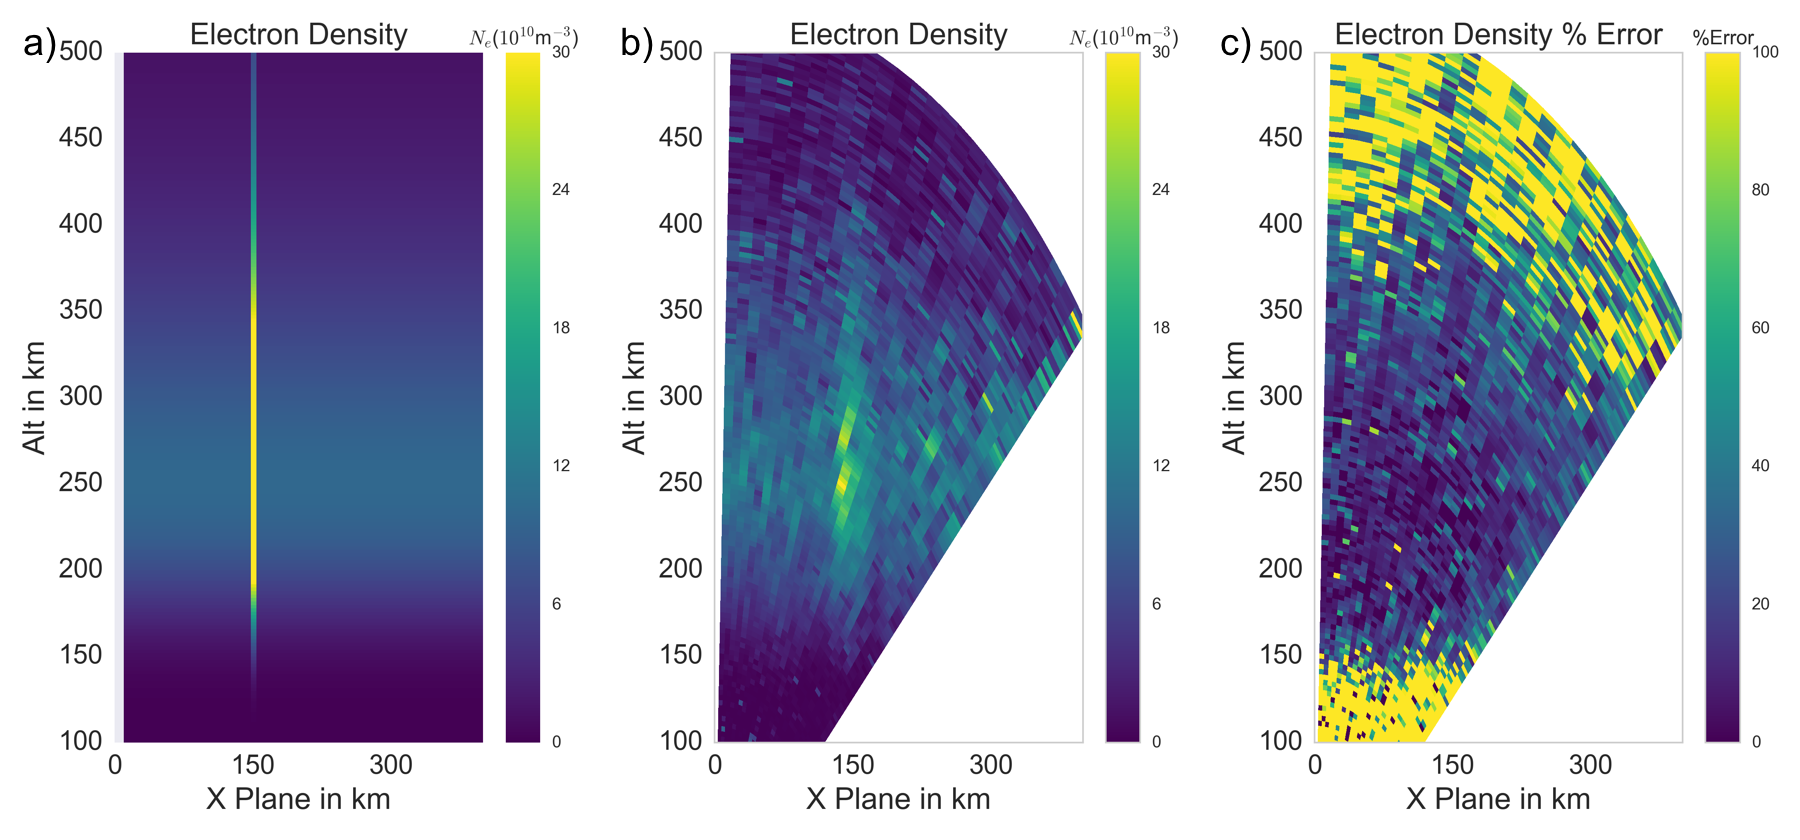
\includegraphics[width=6in]{moving6mins}
\caption{Results of moving enhancement simulation at 600 seconds. a) Input $N_e$. b) Output of simulator with 60 second integration. c) Estimated errors from fit.}
\label{fig:moving10mins}
\end{figure}


\begin{figure}[!t]
\centering
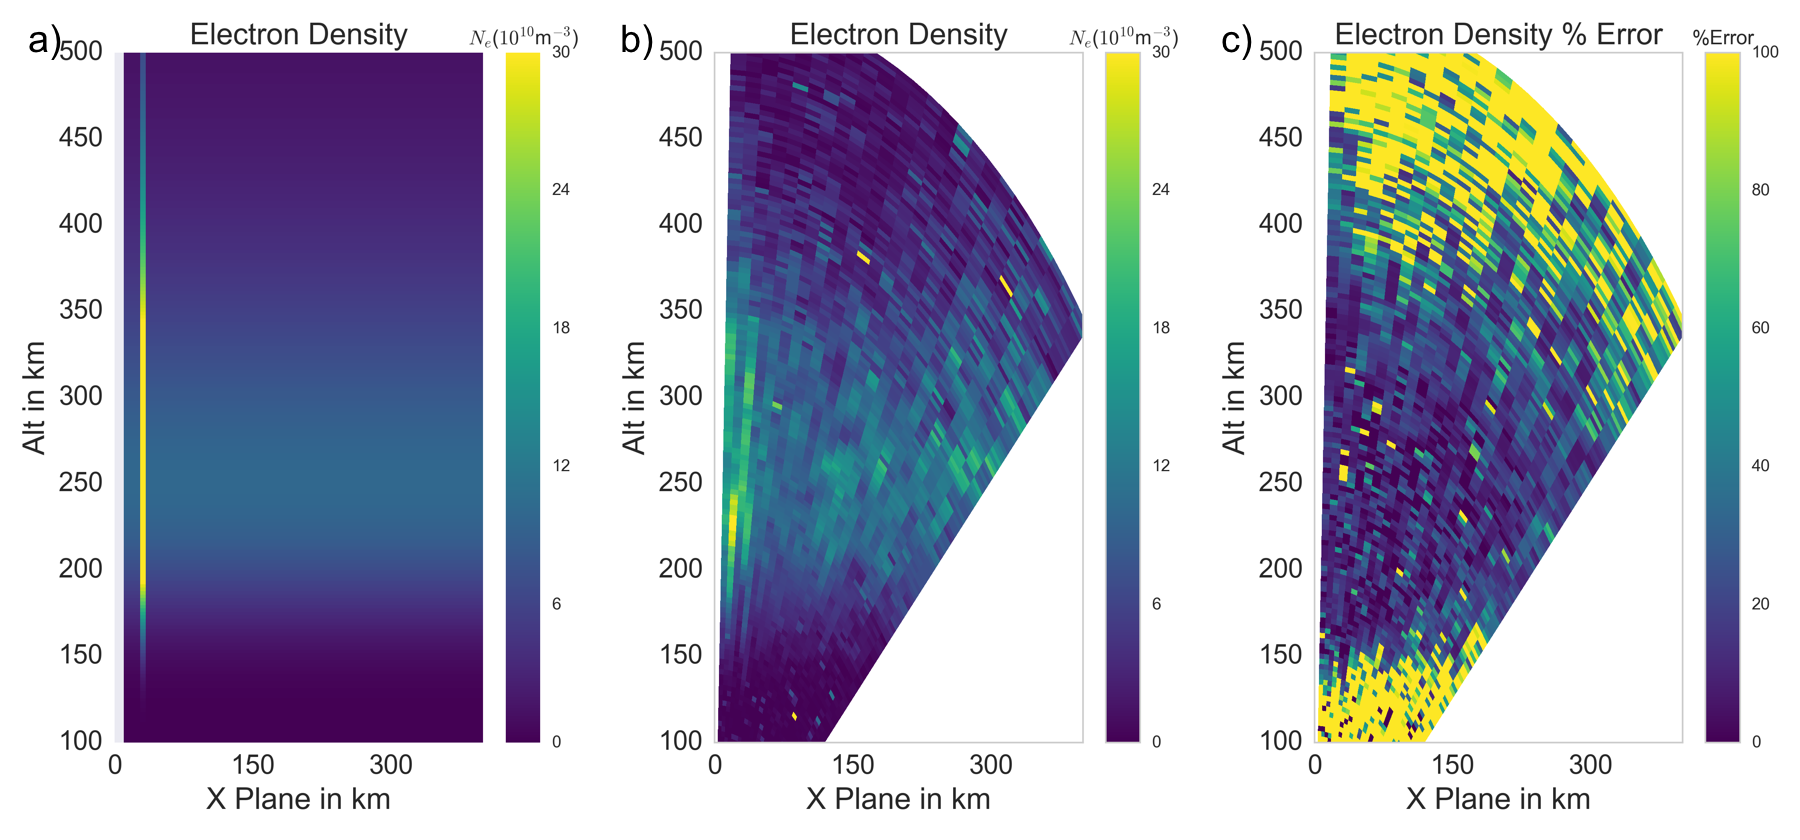
\includegraphics[width=6in]{moving14mins}
\caption{Results of moving enhancement simulation at 840 seconds. a) Input $N_e$. b) Output of simulator with 60 second integration. c) Estimated errors from fit.}
\label{fig:moving14mins}
\end{figure}

This change in the shape of the enhancement can give the impression that its morphology has evolved as it was moving through the field of view of the radar. This could lead to an incorrect interpretation of the physical process taking place, and issue raised by \citep{Dahlgren:2012dq}.   Thus, one must be careful when analyzing these sorts of reconstructions.

Lastly, for this type of simulation, we show an example to demonstrate the situation where a set of two different input parameters can yield qualitatively similar results. For these cases we create electron density enhancements similar to those seen in the high latitude observational study of \citep{Semeter:2005fo} during a poleward boundary intensification event. The sizes of these enhancements are 10 km width and 18 km width. The enhancement in the 10 km width example is 6 times higher than the background while the 18 km width enhancement is 3 times higher than the background.

The input electron density, the fitted electron density and the expected error for the 10 km enhancement can be seen in Figure \ref{fig:moving10all}. The same images for the 18 km wide case can be seen in Figure \ref{fig:moving18all}. Both cases show that electron density enhancements are well above the expected errors.
%% PJE: once again, I cannot see the error morphology here - it just looks like a bunch of pixels at the lowest color level.  Rescale.
%% JPS: I think showing the errors in the same color scale gives the reader an easier time of determining if the results should be trusted. 
%% JLS:  Fine, but all the reader can say from these plots is that the error seems to be below ~12, or ~30%.   DIfficult to discern any color differences below that.
The fitted electron density for both the 10 km enhancement and 18 km enhancement cases show nearly identical results. This simple example demonstrates the possibility to create a non-unique solution in ISR experiments. The results further demonstrate that SimISR can provide useful information in this case, in that it can provide information during the design phase of an experiment that highlight possibilities for ambiguous observational results between two different sets of phenomena. 

\begin{figure}[!t]
\centering
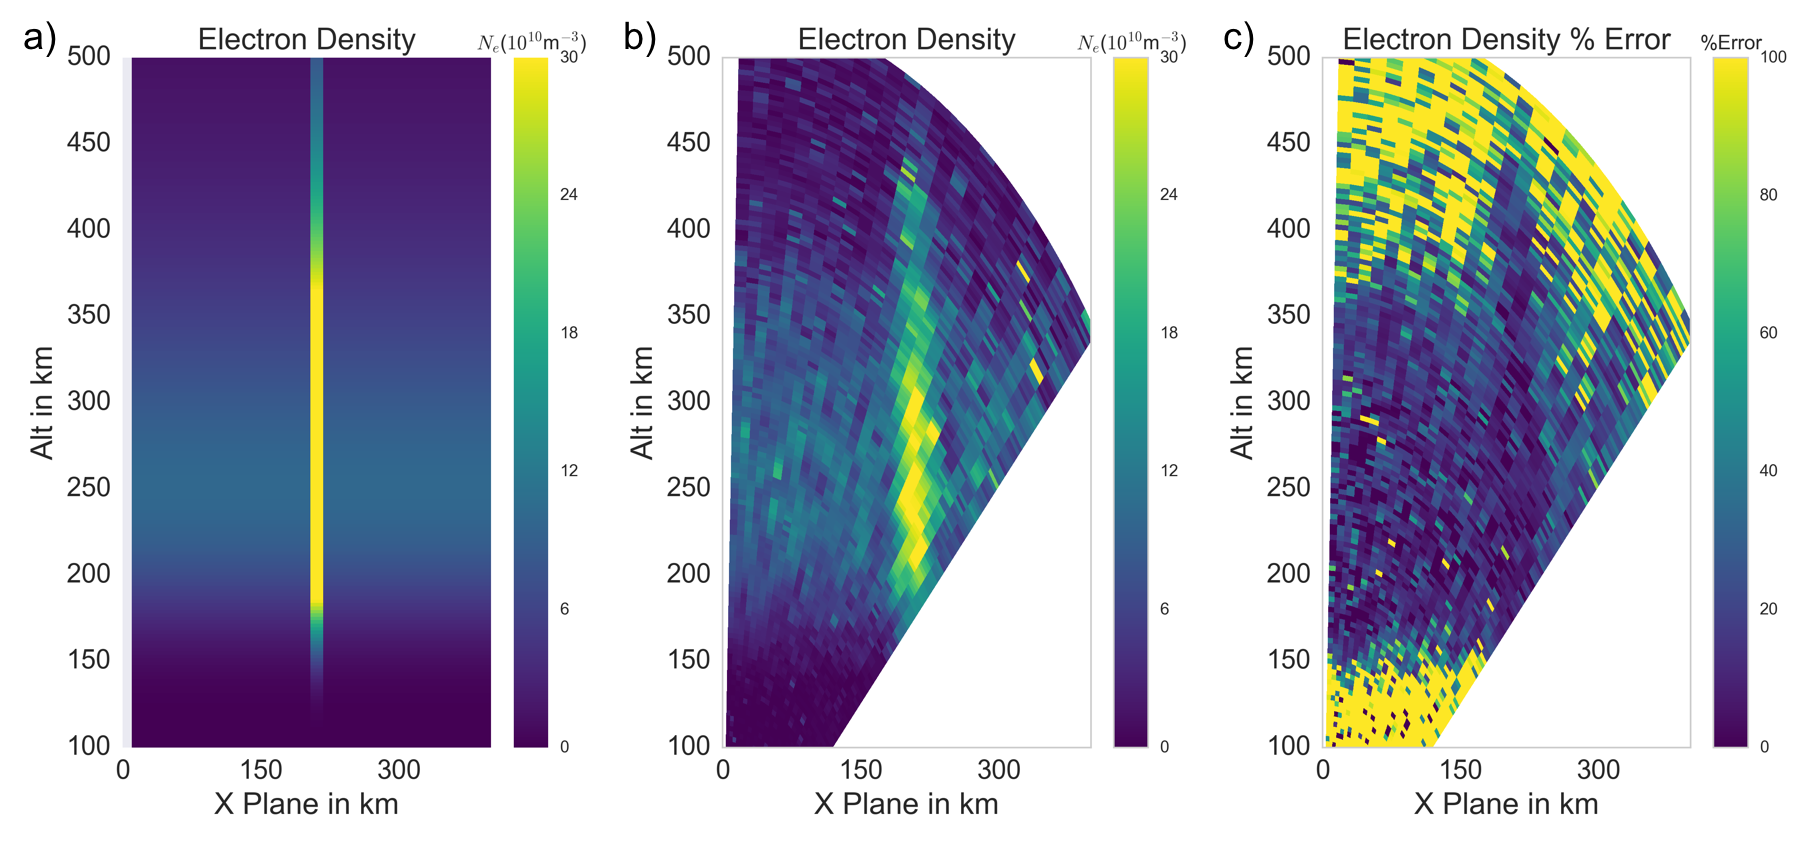
\includegraphics[width=6in]{moving10kminouterr}
\caption{10 km wide enhancement moving simulation at 480 seconds. a) Input $N_e$. a)  b) Fitted $N_e$ with 60 second integration. c) Estimated error from fit.}
\label{fig:moving10all}
\end{figure}

\begin{figure}[!t]
\centering
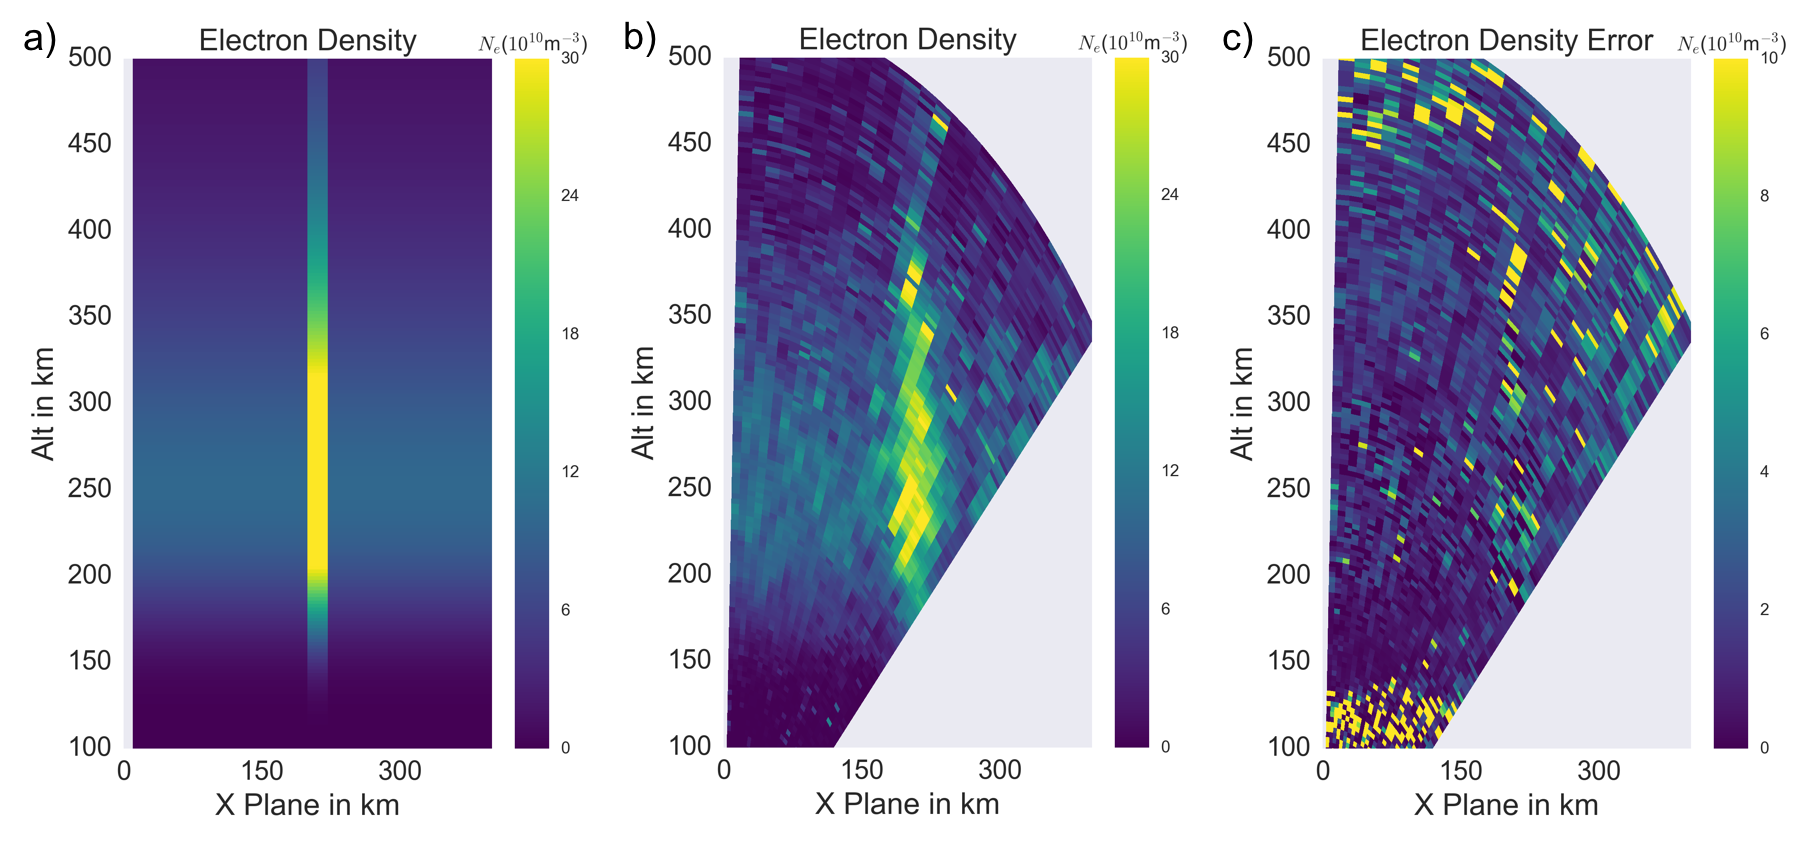
\includegraphics[width=6in]{moving18kminouterr}
\caption{18 km wide enhancement moving simulation at 480 seconds. a) Input $N_e$.  b) Fitted $N_e$ with 60 second integration. c) Estimated error from fit.}
\label{fig:moving18all}
\end{figure}

\subsection{Full Parameter Experiment}
\label{sec:fullparam}
Another SimISR use case employs input plasma parameters derived from the multi-fluid model developed by \citep{semeter:plasmatransport2012}. The specific model run was originally used by \citep{Perry:2015jf} to assist in interpreting measurements of polar cap arcs from the Resolute Bay Incoherent Scatter Radar (RISR). Images of the modeled plasma parameters are shown in Figures \ref{fig:plparamst0} and \ref{fig:plparamst60}. The enhancements in electron density, electron temperature, and ion temperature comprise the self-consistent response of the ionosphere to a field-aligned current system with amplitude .875 $\mu$A/m$^2$.  The source is made to move with respect to the radar at a velocity of 200 m/s (a  value inferred from optical forms observed during this event).  A channel of soft electron precipitation (50-500 eV in energy) is added to the upward current channel, with energy flux consistent with the amount of electron heating seen during the event.  A reasonable objective for a multi-beam ISR experiment could be to validate model predictions of conditions leading to the arc-adjacent density depletion seen in panel a of Figure \ref{fig:plparamst60}.  In this specific case SimISR can be used to assess observability of dynamic plasma structuring and establish confidence intervals on the ISR results.  

%MZ - something looks strange in this figure with Ti - is the a species-averaged or composition-corrected value?  Also I would strongly recommend removing N2+ from this figure, since it doesn't matter at all in this event (viz. it is at least 1000 x lower density than dominant species at all alts.).
\begin{figure}[!t]
\centering
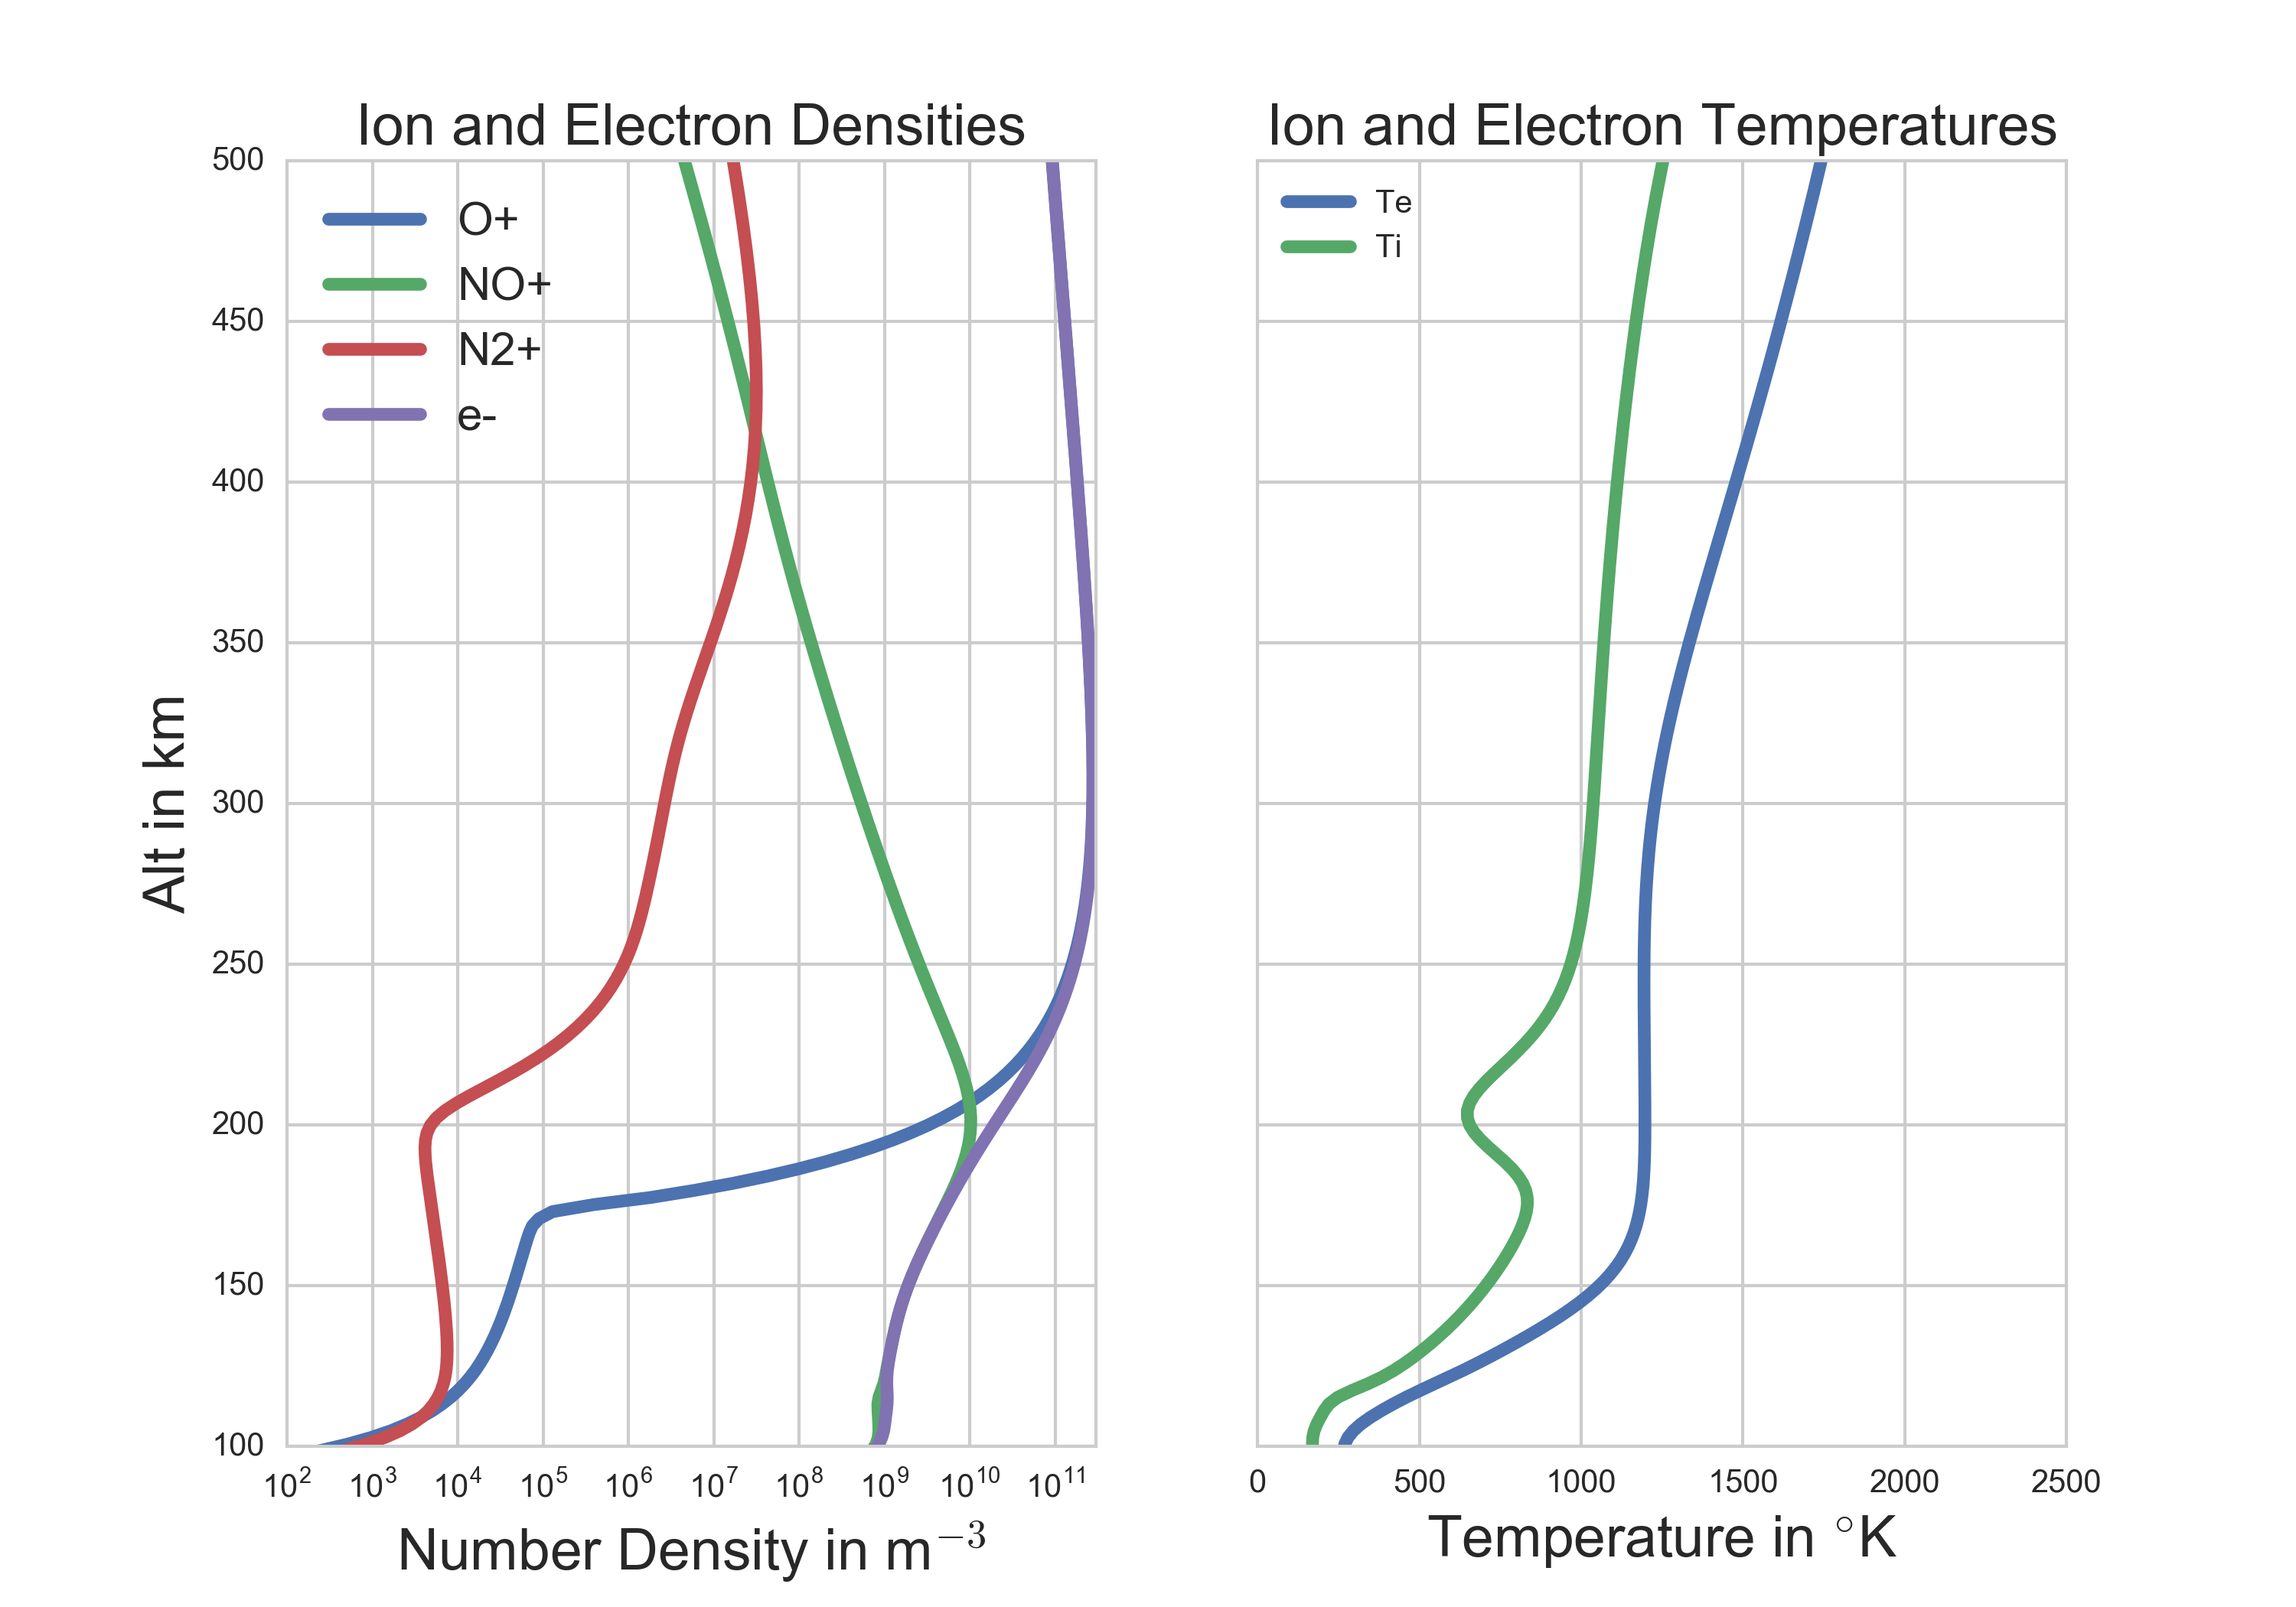
\includegraphics[width=6in]{backgroundallparams}
\caption{Background ionospheric parameters ($N_e$, $T_e$, $T_i$) along with number density of ion species, used for simulations.}
\label{fig:plparamst0}
\end{figure}

%MZ - K or deg. K?  Back in the day they taught us to just use "K", but maybe that has changed...
\begin{figure}[!t]
\centering
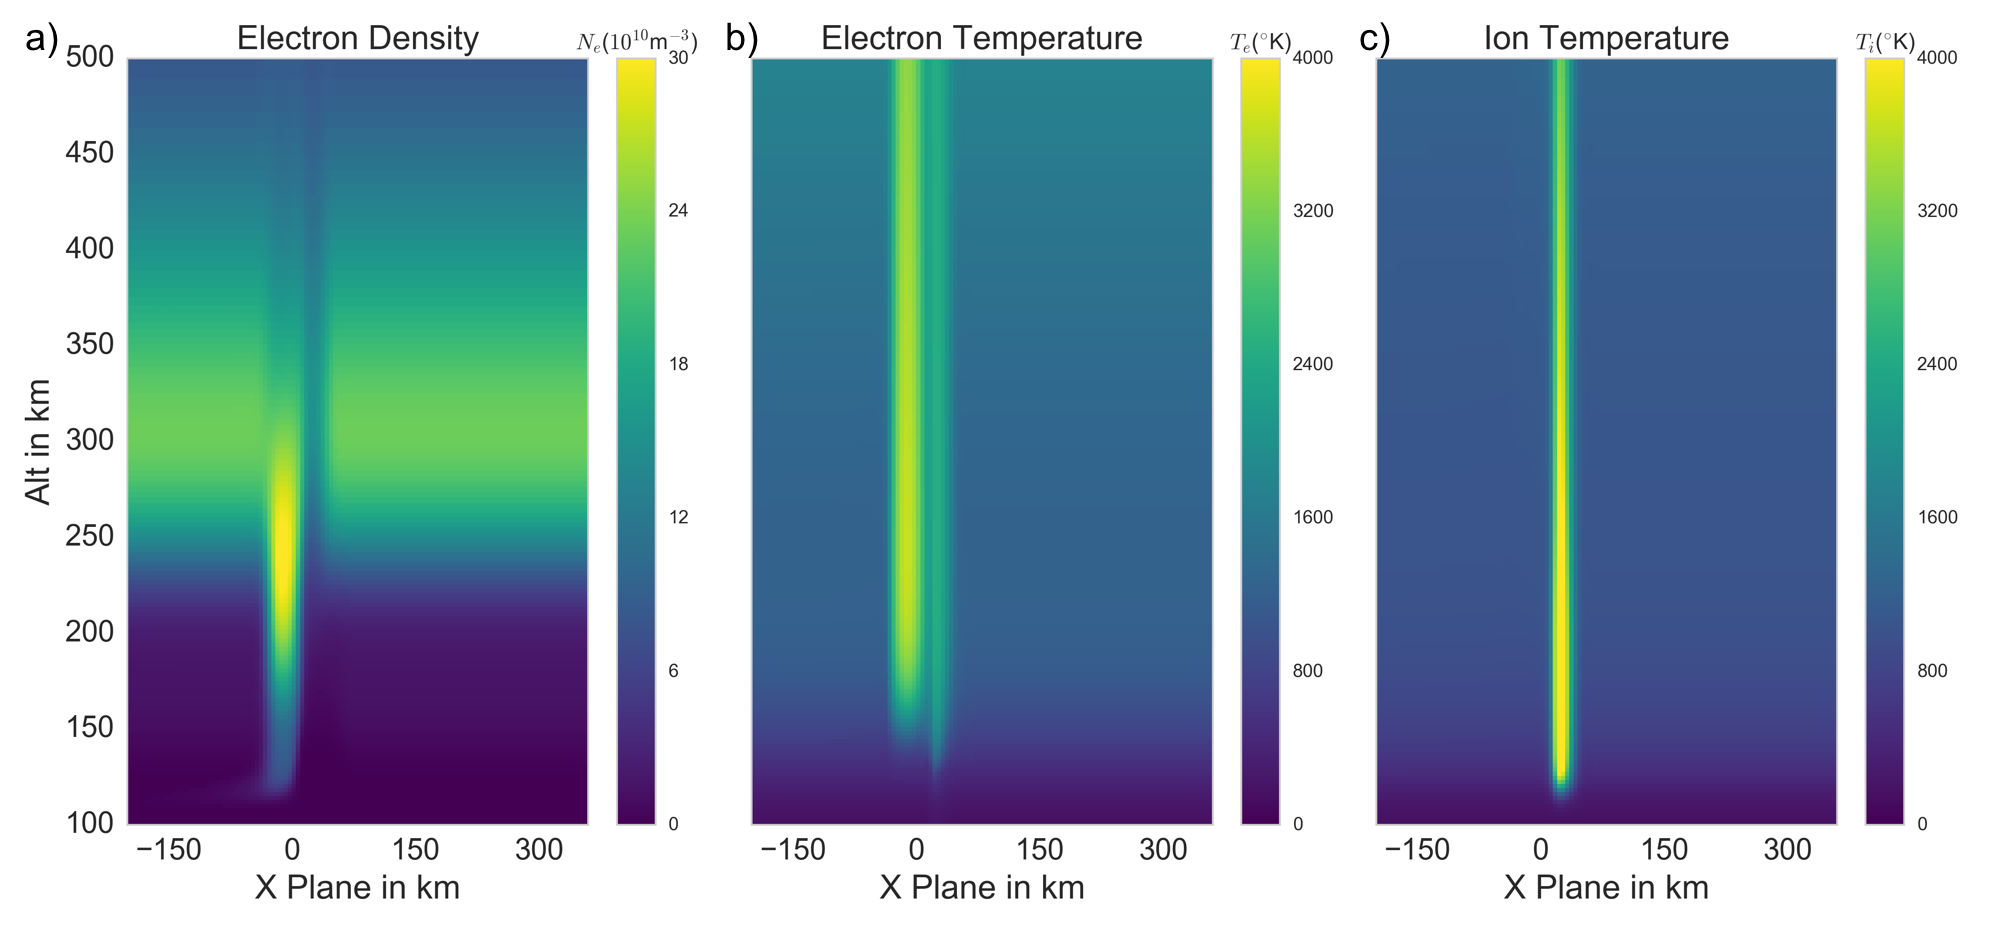
\includegraphics[width=6in]{0960_15_int}
\caption{Perturbations to Figure \ref{fig:plparamst0} due to an imposed current system of .875 $\mu$A/m$^2$ at $t=960$ s, representing an polar cap auroral arc which is sweeping across the field-of-view of the radar at about 200 m/s \citep{Perry:2015jf}.}
\label{fig:plparamst60}
\end{figure}

Using a beam pattern similar to the one seen in the right panel of Figure \ref{fig:backgroundnsamp}, we use SimISR to explore how an electronically scanned ISR may reconstruct this dynamic auroral arc system.  For the purposes of illustration, we use the contrived case where the radar spatial beam pattern is defined to be in the plane of convection.  It is also assumed that the ion species present (particularly their individual masses and relative concentrations) are known. This is a common use case in ISR fitting, as allowing ion concentrations to be free parameters can in some situations allow for non-unique solutions depending on the ion species that are present.  If the fixed, a priori composition ratios between the different ion species are incorrect, this can lead to errors in the final parameter estimates, with ion temperature particularly affected. For the lower F region ionosphere, parameter distortions can occur between 150-250 km where the ionosphere changes from NO$^+$ dominated to O$^+$ dominated \citep{Zettergren:2011ej,Blelly:2010gf}. We also note that as the field aligned current passes through the simulated field, an influx of NO$^+$ appears in the region of rapid ion mass transition for this simulation, potentially violating ion composition assumptions \citep{Perry:2015jf}.
% JOHN:  I can't figure out what the above sentence fragment is supposed to be.
% Josh: I fixed the first sentence of the previous paragraph
% MZ - I'm intrigued by the last sentence.  We do need to explain this a bit better (and I would like to go through the model output from which this is derived to make sure I understand why the model it giving this result)

The output of SimISR in the auroral arc case can be seen in Figure \ref{fig:fplparamst60}. The integration is started at $t=960$ s into the multi-fluid simulation with the plasma parameters shown in Figure \ref{fig:plparamst60}. For this case, a 60 second integration time is used, which for the 27 beam radar experiment set up gives 255 pulses per position. These plasma parameters are linearly interpolated to a Cartesian grid and plotted using the GeoData API \citep{john_swoboda_2016_154533}. Lastly, the expected errors from the fit can be seen in Figure \ref{fig:fplparamst60err}, which are of much lower value that the fitted parameters.
%% PJE: same complaint about expected errors - I can't see anything with the color scale chosen.  Rescale.
%% JPS: See other comments.
We highlight several features in the fitted results. First, the predicted enhancements in electron and ion temperature are clearly observable and well above the expected error. Second, we examine whether the predicted density cavity in the downward field-aligned current region is  detectable. A deepening and broadening region of plasma evacuation is predicted as a self-consistent response to a confined up-down current pair \citep{cran;cavity}.  But it has been unclear whether this prediction can be validated with ISR, since it involves detecting organized channels of reduced backscatter power embedded within a higher density background.
%% PJE: I really don't like the word "coherent" here since it will lead the reader to think of scattering off coherent plasma waves.  I think you should use maybe "organized channels".
%% JPS: Done
%Josh: You didn't have the right citation so I found the best one i could Replaced \citep{write:alfven} with current version
% JOHN:  The Cran-McGreehan paper cited above is the right one, just check that it compiles.
% Josh: It seems to work on my end.
% MZ - I'd be careful attributing the cavities to the Cran/Doe Mechanism.  I think case I think it is a chemical effect (which is, I believe, what Perry et al, 2015 conclude).  However, in general, you would likely not be able to separate the two process with ISR measurements.  
The images shown in Figure \ref{fig:fplparamst60} represent the best case scenario for identifying the presence of this cavity since, at this time, the cavity is nearly co-aligned with one of the beams. 
%For the other cases where the beams are not well aligned with the cavity it becomes much more difficult to observe it due to the range ambiguity being larger than the beam width, making the "filling in" of the evacuated electrons more pronounced. 
Using density measurements alone (panel a) the presence of the cavity is visible, but only marginally so, as it is blended with the adjacent  enhancement produced by the applied precipitation in the upward current channel.  A similar ambiguity exists with the electron temperature result, which could easily be interpreted as purely an effect of heating from soft precipitation.   However, the ion temperature increase in panel b is decidedly narrower than the electron temperature enhancement, offering a possible observable fingerprint for the presence of a confined up-down current pair.  The simulation result illustrates the efficacy of a collective analysis of all plasma state parameters in evaluating the physical mechanism responsible for an observed dynamic.  This is a common approach in data assimilation problems.

%% Fitted Data

\begin{figure}[!t]
\centering
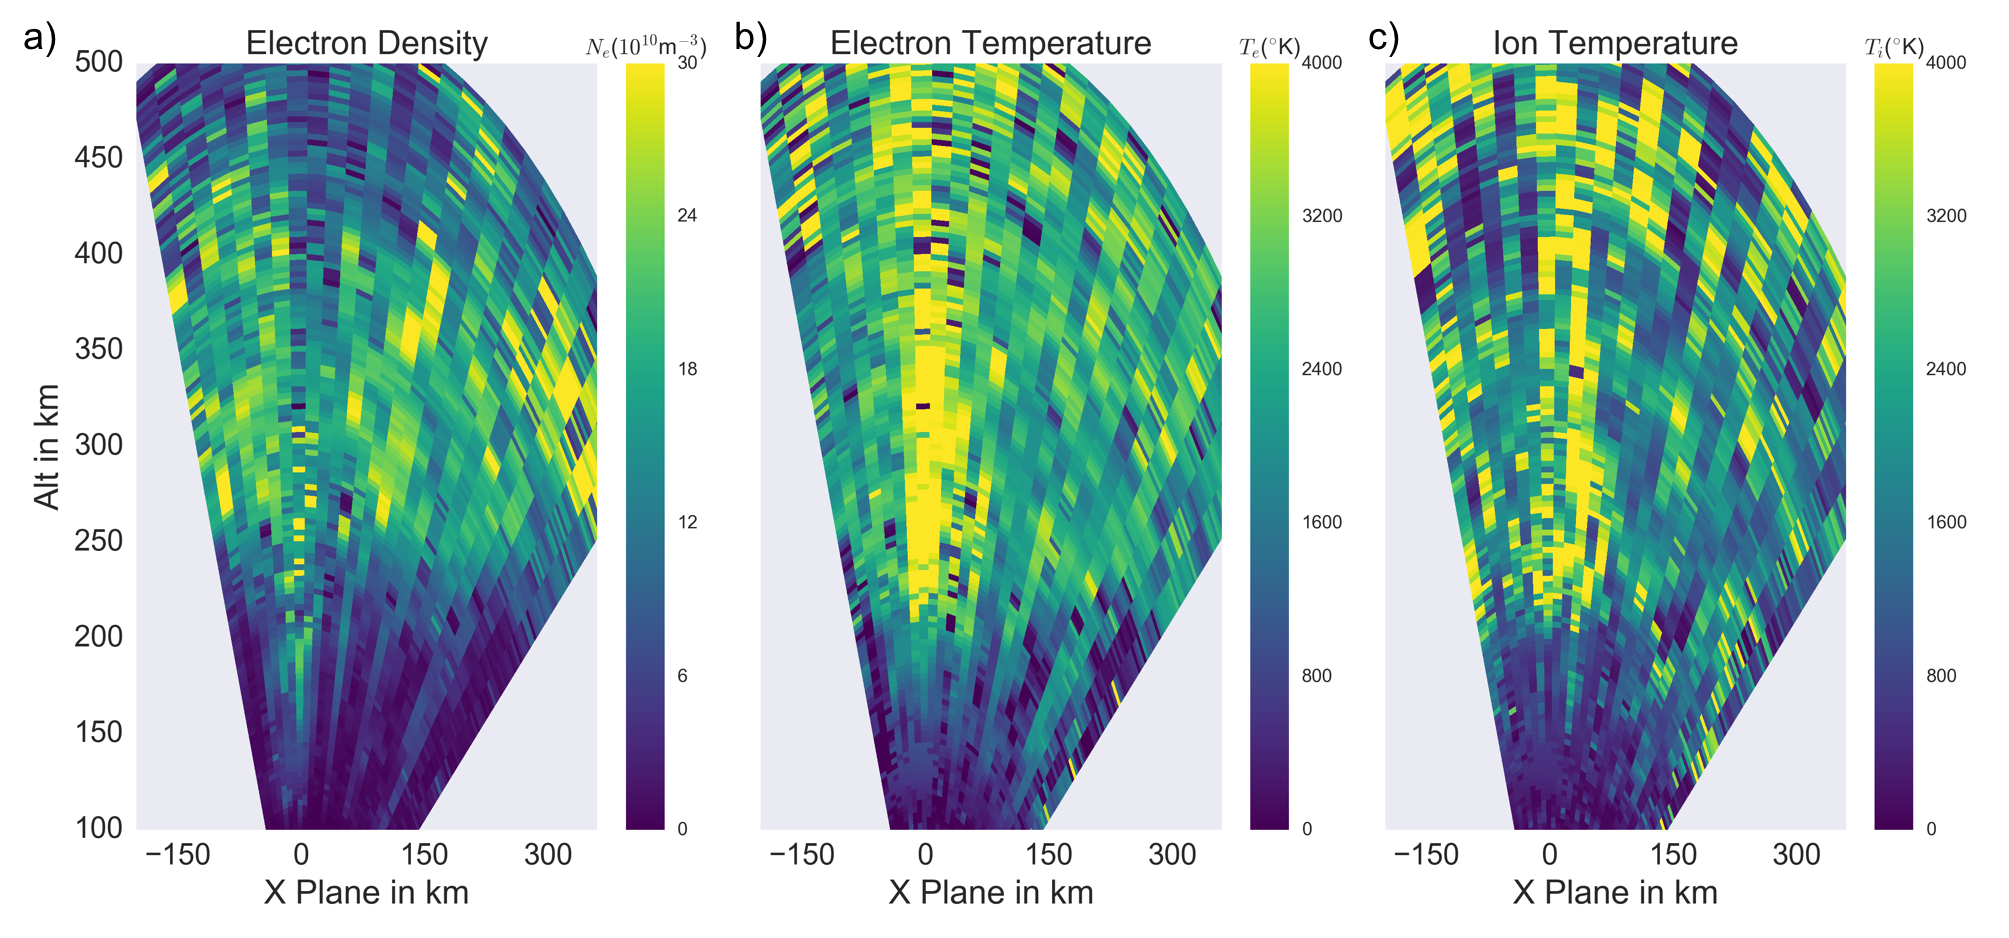
\includegraphics[width=6in]{0960_60_int}
\caption{Fitted Plasma Parameters for the auroral arc case at $t=960$ s with 60 second integration.}
%JOHN:  need to label these A,  B, C
%Josh: I have the parameter type in the title so that should be enough.
\label{fig:fplparamst60}
\end{figure}

\begin{figure}[!t]
\centering
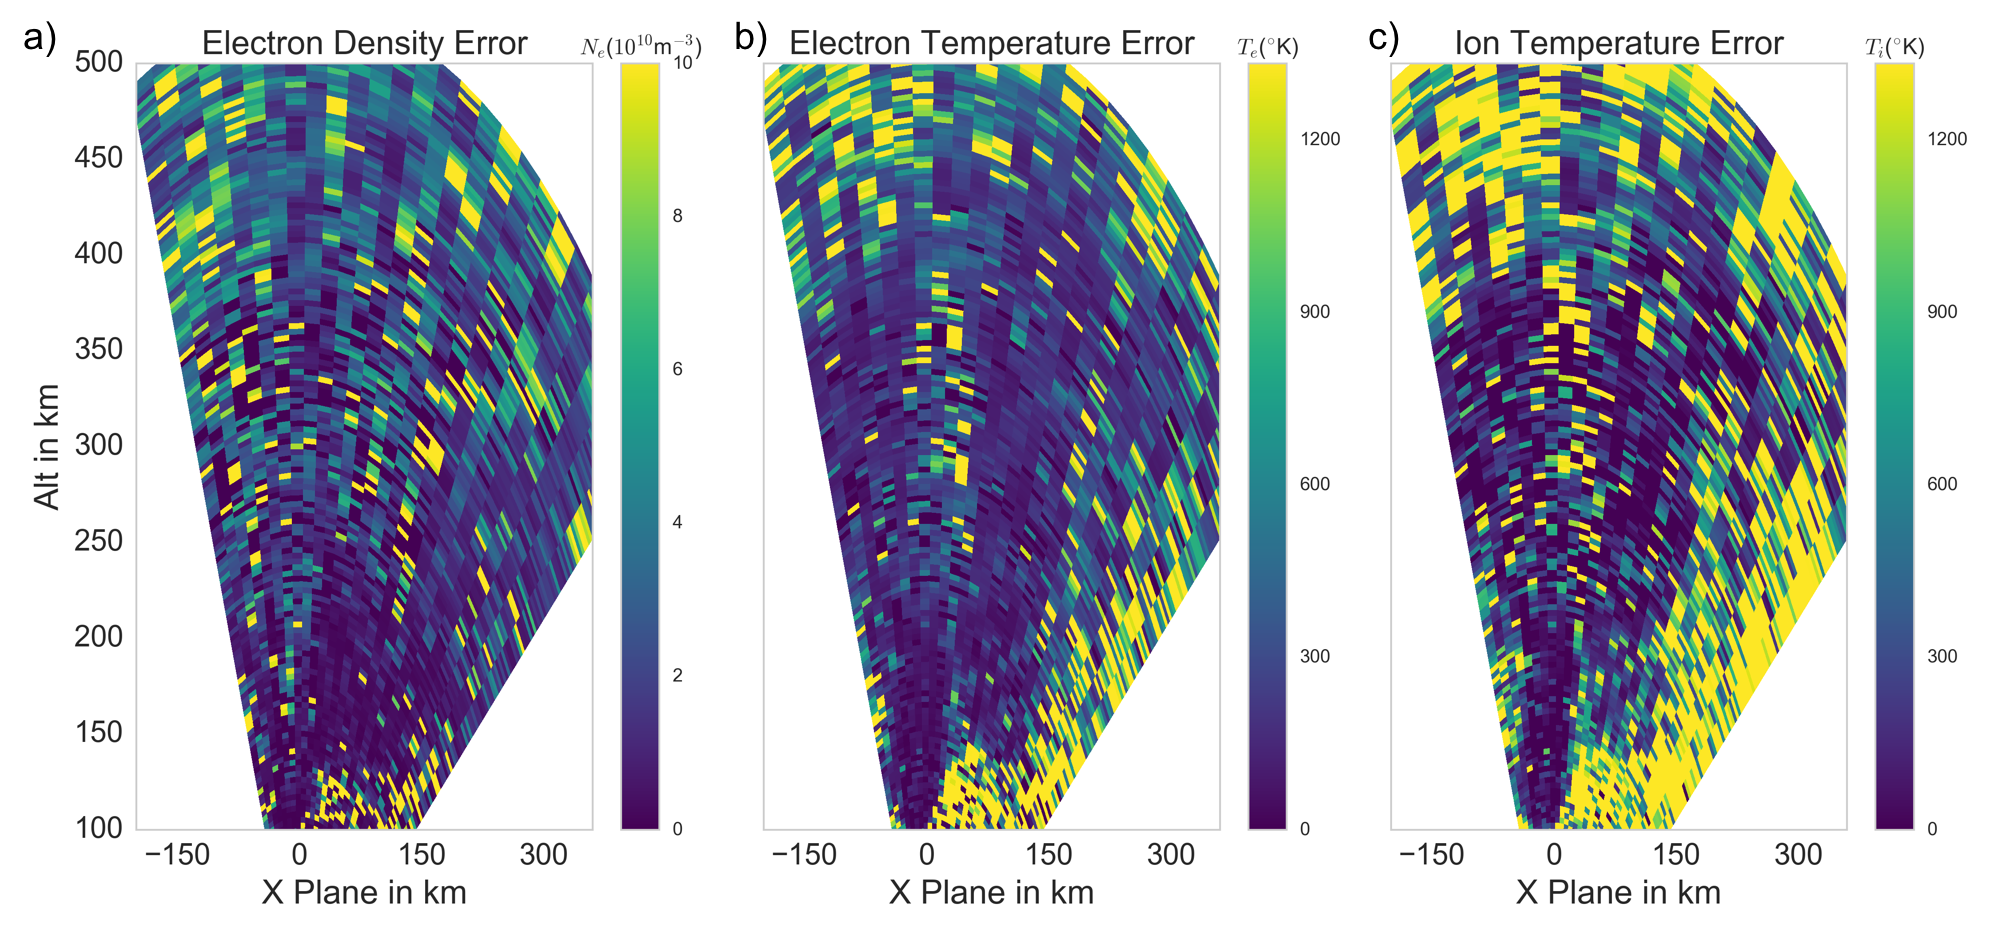
\includegraphics[width=6in]{0960_60_int_err}
\caption{Estimated errors from fitted Plasma Parameters for the auroral arc case at $t=960$ s with 60 second integration.}
\label{fig:fplparamst60err}
\end{figure}

\subsection{Full 3-D Reconstruction}

%JLS:  Rewrote this section
A common application of ESA-based ISR's (PFISR and RISR) is to create three-dimensional time-dependent visualizations of  dynamically evolving parameter fields \citep{Nicolls:2007ie,Semeter2009738,semeter:jgr2010,dahlgren2012di}.   Such results are visually compelling but, as yet, there has been no framework advanced to evaluate uncertainties and potential artifacts in these interpolated views, or to apply these results in a quantitative comparisons with predictions from physical models.  The state of modeling of the coupled magnetosphere-ionosphere system has progressed considerably in recent years. In particular, hybrid fluid-kinetic models are able to make detailed  predictions of small- and meso-scale processes underlying global-scale system behavior \citep{damiano;jgr2005,semeter:plasmatransport2012,akbari:jgr2016}.  Simulation will enable us to do formal hypothesis testing on these predictions, which often involves the detection of subtle space-time variations in a parameter field.

As an example, SimISR was driven using plasma parameters computed from a three-dimensional version of multi-fluid model \citep{zettergren2015dynamics} used to test simISR in the previous section. The parameter distributions represent the self-consistent ionospheric response to a 0.65-$\mu$A/m$^2$ field-aligned current (FAC) that is turned on at model time $t=0$, and remains constant in time.  The Region 1-like FAC creates large enhancements in ion temperature due to frictional heating, and also causes smaller amplitude enhancements (and depletions, as before) in electron density.
%MZ - Just checking this isn't the Perry event anymore, right?  I ask because I think I've sent 3D results from that one as well at some point, but I know I've sent you other stuff, as well.

The spatial domain is sampled using the beam pattern and sampling lattice shown in Figure \ref{fig:3dsampling}. This is a 121 beam pattern similar to the one used by \citep{Semeter:2008hs}. For this simulation the data are integrated over 315 seconds which, with a 8.7 ms IPP and the current beam position, yields 300 pulses per position.
%% PJE: fill in the XXX
%% JPS: Filled in
After the data were fitted, a three-dimensional natural neighbor interpolation was performed \citep{Sukumar:nn2001} and the results
%% PJE: natural neighbors? Do you mean nearest neighbors?
%% JPS: Natural neighbors is another interpolation scheme and we've used it in the past for interpolating 3-D reconstructions.
%% JLS: Added natural neighbor citation
plotted using the GeoData API \citep{john_swoboda_2016_154536}.

\begin{figure}[!t]
\centering
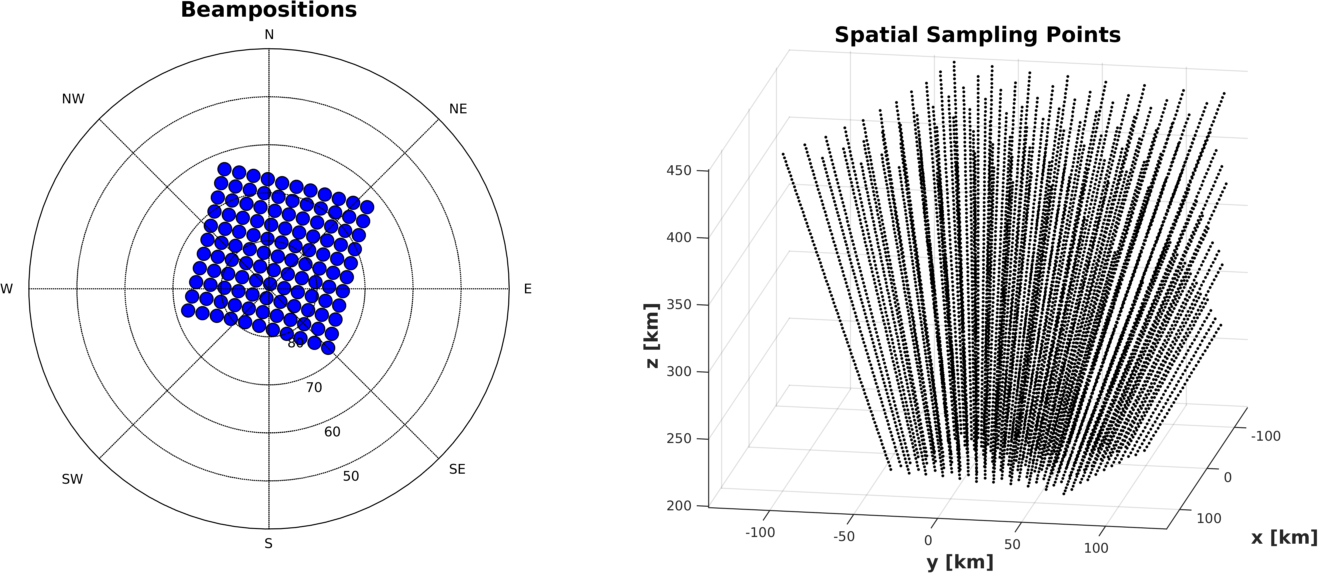
\includegraphics[width=6in]{Sampling3d}
\caption{The beam pattern used in angle space and the resulting 3-D spatial sampling pattern used for the three dimensional SimISR use case simulation.}
\label{fig:3dsampling}
\end{figure}

The input plasma parameters and the results of SimISR simulation are summarized in Figure \ref{fig:3dparams}.  For the selected configuration, the reconstructed density and ion temperature fields capture the predicted spatial variations reasonably well, providing confidence that this experimental configuration would result yield a positive detection of the spatial variations predicted by the applied FAC.  Reconstruction of the electron temperature enhancement (which is derived from a higher-order moment of the ISR spectrum) is less conclusive. This highlights the important point that variance is parameter dependent. In this case, SimISR informs us that, for this FAC and this experimental configuration, a negative result for $T_e$ comparison is not sufficient grounds to discount the model prediction.  A further refinement of the experiment might yield a positive result.

\begin{figure}[!h]
\centering
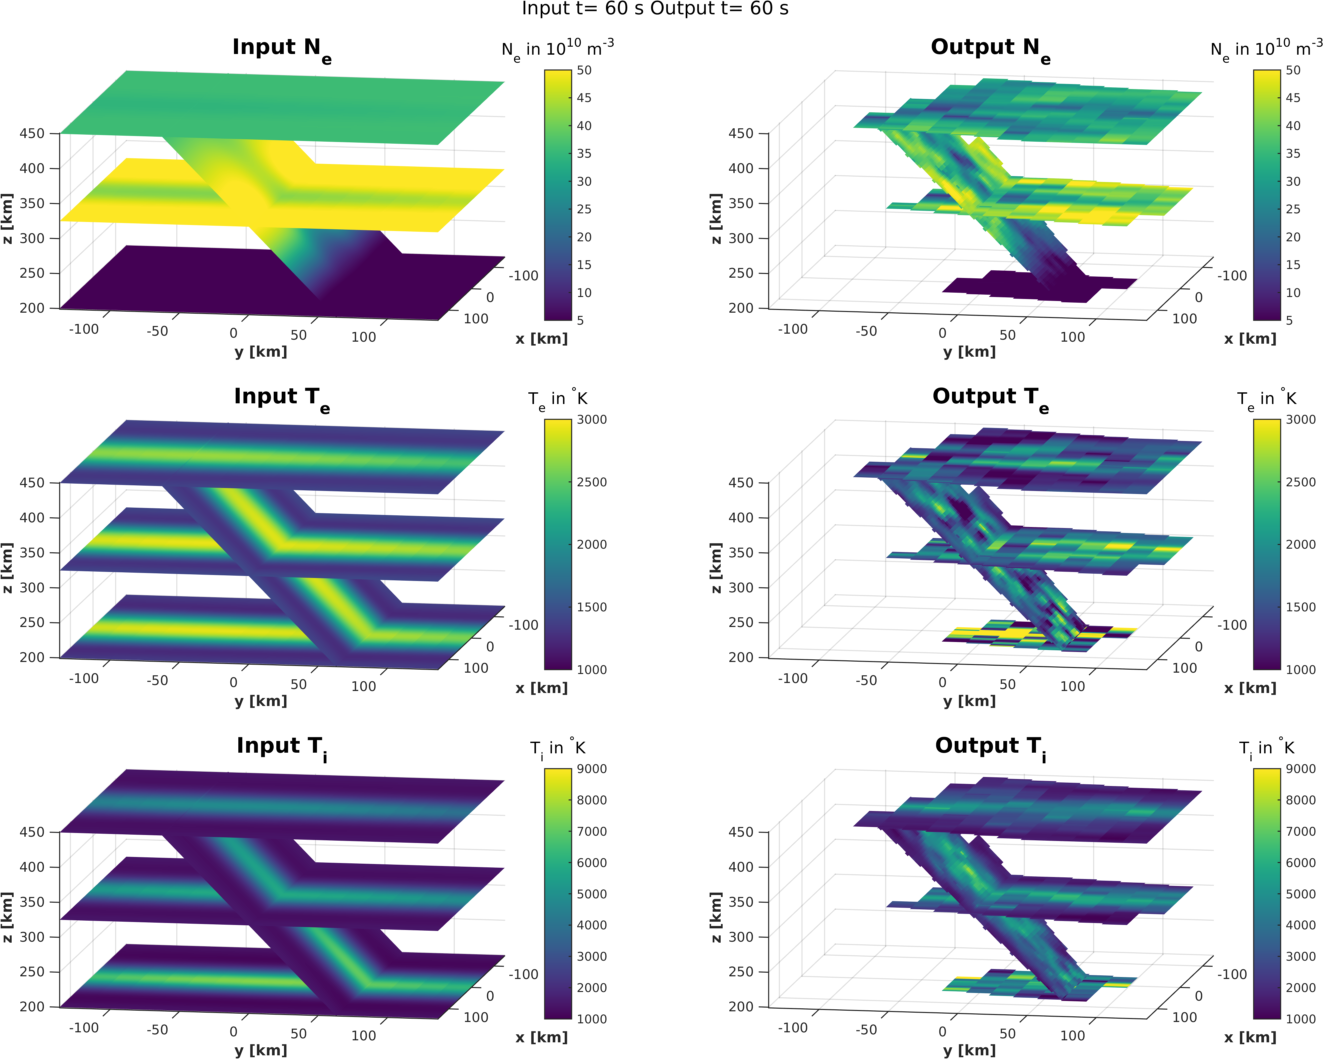
\includegraphics[width=6in]{60_60}
\caption{Input and output of full 3-D reconstruction of plasma parameters.}
\label{fig:3dparams}
\end{figure}

The sampling pattern picked for this simulation was chosen to get as dense a set of non-overlapping beams as possible.  This has been the general objective for several previous volumetric imaging experiments.
%% PJE: is this the main point? Or not?
%% JPS: This mode was designed off of a previous experiment although it is a very dense pattern.
The overall phenomena varies over a much larger area, so there is an obvious trade off between sampling density and the support region. These sorts of simulations can help experiment planners to understand these trade offs and possibly yield to innovative sampling stratagems for specific phenomena. 

\section{Summary}
This chapter showed the methodology behind the SimISR software package which can create synthetic ISR data. This simulator can be used in a number of different ways and is available to the research community. SimISR shows good correspondence with real data but there are difference which can be attributed to specific choices made for the specific simulation shown and variations in data processing between PFISR and SimISR for estimating the parameters.